
\chapter{Introduction}
\label{sec:Introduction}

\label{sub:figures}

\begin{figure}[ht]
	\begin{center}
		\begin{subfigure}[b]{0.33\textwidth}
			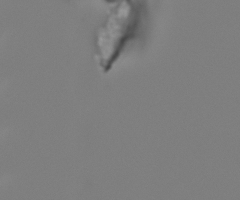
\includegraphics[width=\textwidth]{thesis-template-master/images/(1095).png}
			\caption{Debris}
			\label{fig:Debris}
		\end{subfigure}
		\begin{subfigure}[b]{0.33\textwidth}
			\reflectbox{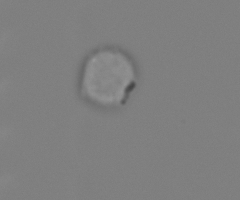
\includegraphics[width=\textwidth]{thesis-template-master/images/(635).png}}
			\caption{Out of Focus}
			\label{fig:Out of Focus}
		\end{subfigure}
		\begin{subfigure}[b]{0.33\textwidth}
			\reflectbox{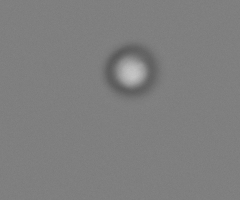
\includegraphics[width=\textwidth]{thesis-template-master/images/(1672).png}}
			\caption{Lighting Artifacts}
			\label{fig:Lighting Artifacts}
		\end{subfigure}
		\begin{subfigure}[b]{0.33\textwidth}
			\reflectbox{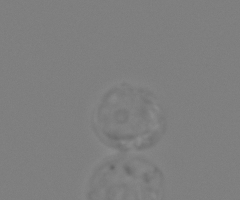
\includegraphics[width=\textwidth]{thesis-template-master/images/(1112).png}}
			\caption{Outside FOV}
			\label{fig:Outside FOV}
		\end{subfigure}
		\begin{subfigure}[b]{0.33\textwidth}
			\reflectbox{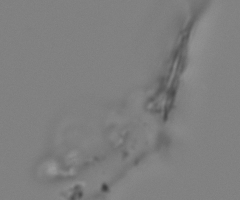
\includegraphics[width=\textwidth]{thesis-template-master/images/(1684).png}}
			\caption{Contaminated}
			\label{fig:Contaminated}
		\end{subfigure}
		\begin{subfigure}[b]{0.33\textwidth}
			\reflectbox{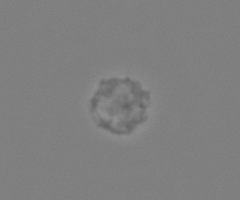
\includegraphics[width=\textwidth]{thesis-template-master/images/hd3 (56).png}}
			\caption{Good Cell}
			\label{fig:Good Cell}
		\end{subfigure}
	\end{center}
	\caption{Six Typical Cell images on original Sezary Syndrome data set. Only Good Cell can provide useful Morphology characteristics for further classification.}
	\label{fig:lennas}
\end{figure}

Sezary Syndrom is an aggressive form of cutaneous T-cell lymphoma that is characterized by presence of tumor T-cells with abnormal nucleus morphology in the peripheral blood. The easy and precise detection of malignant cells in the blood of patients with Sezary Syndrome is of important diagnostic, prognostic and therapeutic value, and is essential for disease monitoring under treatment\cite{b6}\cite{b7}. The severe limitations of manual microscopic identification of tumor T-cells have led to the implementation of flow cytometry-based diagnostic assays. Currently, the loss of cell surface markers, such as CD26, CD27 and CD7, on malignant T lymphocytes remains one of the most consistent features and is routinely used in the diagnostic workup \cite{b12}, although their specificity and especially sensitivity, must be interpreted with caution \cite{b11}. We plan to circumvent the challenges involving the definition of molecular diagnostic markers and rather aim at re-surging morphology-based diagnosis of hematological malignancies through an automated procedure, integrating imaging flow cytometry and deep learning as a route to, ultra-high throughput and sensitive diagnosis.
 
\label{sub:figures}
\begin{figure}[ht]
	\begin{center}
	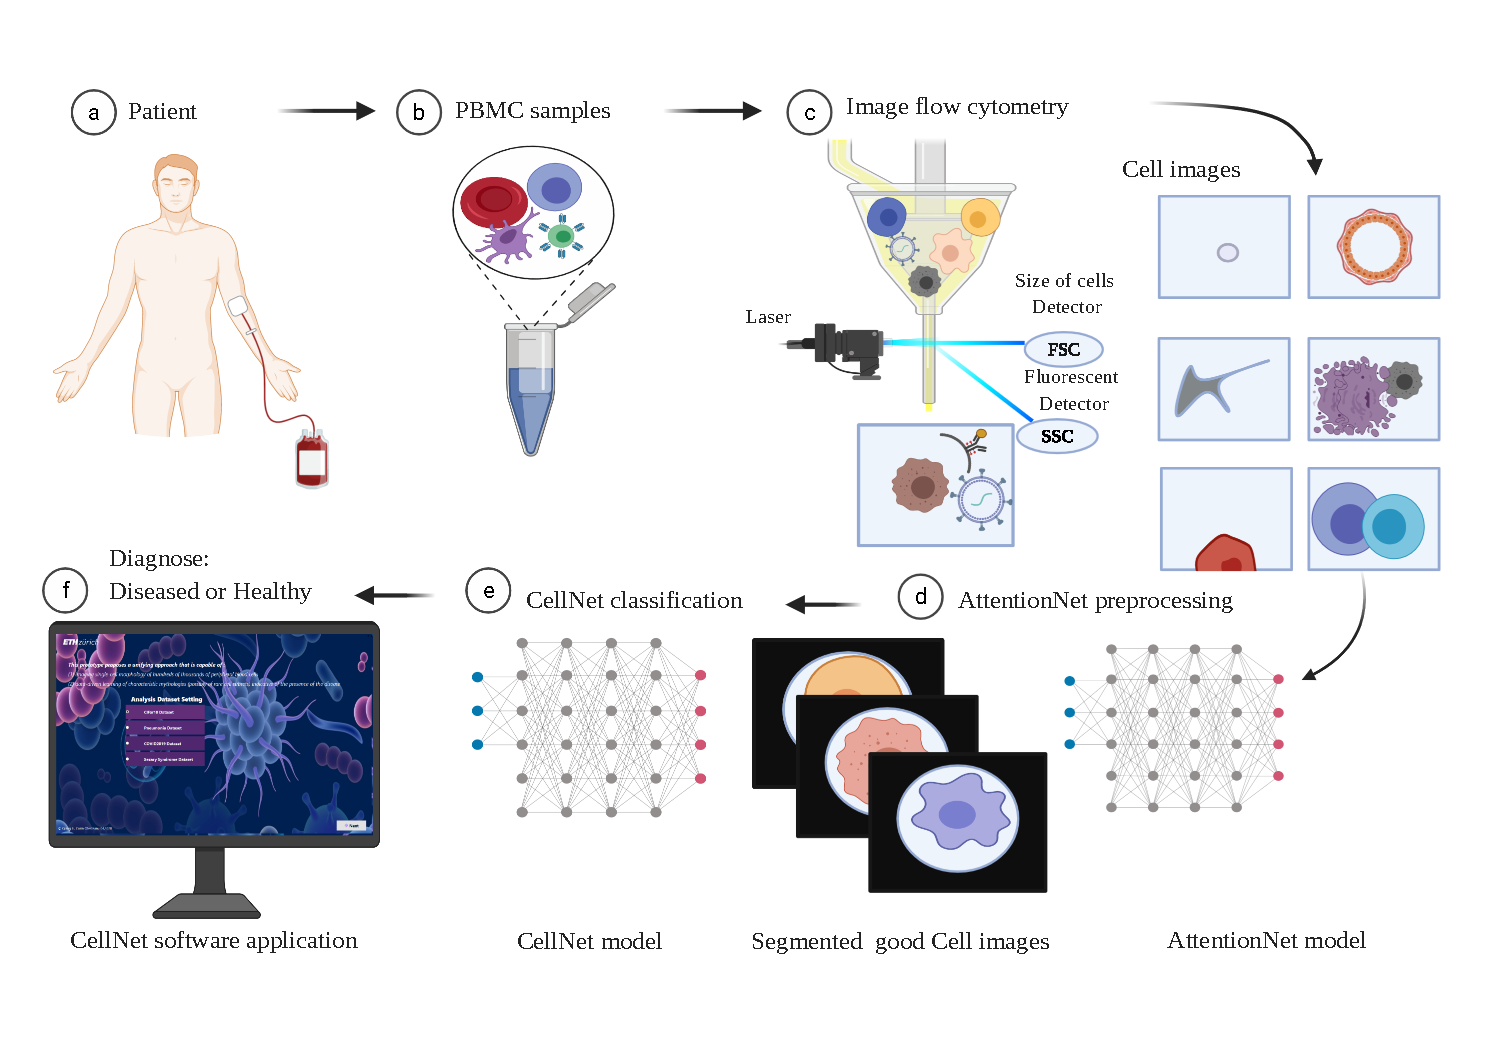
\includegraphics[width=\textwidth]{thesis-template-master/images/general workflow2.pdf}
	\label{fig:lenna}
	\end{center}
	\caption{General Workflow of Proposed Project. After Image Flow Cytometry (Morphological identification of tumor T-cells in the blood), those generated images can be categorized into 6 typical classes: lighting artifacts, out of focus cell, debris, contaminated cell, outside FOV cells  and multiple cell concatenated together. Using AttentionNet as a automatic detector and segment-or, we can filter out most of the artifacts in the images and only keep the morphological characteristics of the cell for CellNet classification. CellNet only has 8 novel Ghost module layers. CellNet software includes a total of 5 interfaces, 25 buttons, 10 user prompt functions and inherits 12 algorithms with the integration of 4 data sets.}
	\label{fig:lennas}
\end{figure}



In the first step, CellYolo approach has been developed to automatically annotate and segment cell types to single-cell images obtained from imaging flow cytometry experiments. These approach is based on deep learning paradigms that have emerged as a disruptive alternative to engineering-based techniques, which easily lead to a large amount of impure labelled data, and requires more resources and time. CellYolo as an efficient and accurate object detector emphasizing on small target, inherited the characteristics of the real-time detection of the YOLO network\cite{b33}, and at the same time avoided the low accuracy of the YOLO network in detecting small objects. Inspired from the YOLOv3-tiny network ,the K Means++ algorithm is an efficient approach of data pre-processing\cite{b18}. Experimental results demonstrate that CellYolo is not only a cost efficient solution for practical application( Labeling/Segmenting each image takes only 0.25 seconds in Intel CPU), but also an effective way of improving accuracy of object classification. We reproduced and integrated nearly 20 classic computer vision algorithms and test the performance with/without CellYolo preprocessing. With help of CellYolo preprocessing, the improvement based on state-of-the art algorithms in terms of Top-1 val-acc has been verified.

Once segmented, we proposed CellNet for Sezary Syndrom Cell / Healthy Cell classification. We applied similar Residual layer to forward and enable deeper neural network and follows the basic architecture of ResNet18 and GhostNet for its superiority \cite{b19}\cite{b20}. Replaced all the ResNet18 \cite{b20} point-wise convolutional layers (in total, 18 layers ) with Ghost Bottleneck \cite{b19}. In additional, we adopted the SE layers from Squeeze-and-Excitation Networks \cite{b24} to enhance useful features, scaling less inhibiting features map. In each ghost module, we first take pointwise conv to get a few intrinsic feature maps, then we utilized the linear cheap transformation such as depth-wise conv or affine transformation and wavelet transformation, as suggested by GhostNet\cite{b19}, here the depthwise conv was used.
Despite its simplicity (only 8 layers ghost module) and lower parameters(1/4 weights than ResNet18\cite{b20}, 1/2 weights than GhostNet\cite{b19}), CellNet establishes a new state-of-the-art on Sezary Syndrome Dataset (95.638\% Top-1 accuracy) and CIFar10 ( 90.051\% Top-1 accuracy)\cite{b21}. Moreover, the same method is also very competitive against recent leading Supervised approaches on Pneumonia Dataset (91.785\% Top -1 accuracy), where Inception V3 adopted after 7000 epochs reaches only 88.0\%\cite{b38}.

The remaining sections of this paper are organized as follows: Section 2 outlines some of the most relevant  prior work in medical image classification and segmentation including a short introduction about YOLOv3 \cite{b33} algorithm, the most important intuition of Residual learning, and recently invention of Ghost module.
Section 3 introduces our proposal. Section 4 presents experimental verification  and visualization on different benchmark dataset to validate the effectiveness of the proposed models and illustrates several ablative studies.Finally, conclusions are summarized in Section 5.

Our contributions. We proposes a unifying approach that is capable of (1) imaging single-cell morphology of thousands of peripheral blood cells and (2) data-driven learning of morphological characteristics, which are indicative of the presence of the disease.
Inspired by leading SOTA model, such as Deep Residual Learning\cite{b20} and Ghosts Net\cite{b19}, we proposed CellNet. Instead of stacking lots of point-wise convolutional layers and takes huge amount of convolutional manipulations, we can avoid the redundant feature maps by taking cheap operation. CellNet is originally designed for Sezary Syndrome Dataset and we provide comprehensive empirical evidence showing that CellNet has 1/4 weights than ResNet18 \cite{b20} and best classification performances on 
several other benchmarks such as CIFar10 \cite{b21} (92.451\% Top-1 accuracy), Pneumonia Dataset\cite{b38} (91.785\% Top-1 accuracy) and Sezary Syndrome Dataset (95.638\% Top-1 accuracy).
In addition, we purposed AttentionNet Network as an automated data pro-processing tool which provides a new intuition for object recognition, eliminating noise artifacts out of the image precisely can effectively improve the classification performance of many SOTA networks. Instead of manually labeling a large amount of data after Image flow cytometry and PBMC samples \cite{b12}, it is possible to automatically label an object with an accuracy of 88.64 \% in 0.25 seconds by using AttentionNet. 

We also produced the first COVID-19 Chest Xray/CT Dataset containing nearly 2,000 Xray/CT images (nearly 1,500 Healthy Xray/CT images and nearly 500 COVID-19 infected Xray/CT images). Experiments conducted on COVID-19 Datasets also demonstrated that the proposed CellNet is an impressive alternative of current baseline models, and our CellNet (94.719\% in Top-1 accuracy) outperforms the GhostNet\cite{b19} (92.739\%  in Top -1 accuracy) and other leading models. In addition, we developed a software application for potential diagnosis, which integrated with 12 leading SOTA models, including our CellNet. All code is available at \textit{https://github.com/Johnny-liqiang/CellNetUML}.



%3D data representations have been studied independently in their main field of application so far. In this thesis, however, we explore the potential of combining geodesic and Euclidean convolutions on point clouds and meshes simultaneously in the task of 3D semantic scene segmentation. In Figure 1.2, we illustrate our intuition that geodesic and Euclidean convolutions focus on different aspects of feature learning. Geodesic convolutions define proximity in terms of mesh neighbors reach￾able within  hops on the mesh. When applying convolutions on this neighborhood, we explicitly learn features focusing on the surface structure of the scene. For instance,in Figure 1.2a, the geodesic receptive field of the green center point just comprises vertices of the geodesically close chair surface. It therefore neglects geodesically remote but spatially close vertices of the table. Hence, we assume that geodesic convolutions are more likely to learn feature representations for object shapes.

%Contrastingly, Euclidean convolutions focus on the Euclidean proximity of vertices in terms of nn or radius neighborhoods in 3D space. They enable an information flow between geodesically disconnected parts of the scene and therefore, we assume that they learn the interaction between objects. For example, in Figure 1.2b, the convolution does not generate features only based on vertices of the chair but also based on the geodesically remote table. We assume that this contextual information helps to distinguish shape-wise similar classes such as chair and armchair. Concludingly, we pose the question if a combination of geodesic and Euclidean convolutions brings a significant benefit for the task of 3D scene segmentation. For this purpose, we have developed a simple yet effective multi-scale architecture called DualConvNet which combines Euclidean and geodesic convolutions in a parallel manner over multiple scales. Special provisions have been taken to guarantee the modularity of the architecture such that all effects are measurable in order to answer the research question in the ablation study experimentally.

%Our approach is mesh-centric in that sense that it consumes meshes as a half-edge data structure as well as defining (un-)pooling operations in terms of mesh simplification algorithms. This design decision is necessary to ensure a mesh structure in deeper network layers such that geodesic convolutions are well-defined. We therefore extend vertex clustering [RB93] and Quadric Error Metrics (QEM) [GH97] as two well-established algorithms from the geometry processing domain such that they can pool and unpool vertex sets from consecutive hierarchy levels. Pooling Trace Maps constitute this extension which comprises a look-up dictionary approach for obtaining pooled representatives in constant time. In order to make QEM pooling applicable for large-scale meshes, we finally present a novel sampling strategy for radius neighborhoods called Random Edge Sampling (RES) which outputs a sample set which guarantees an upper limit of a predefined expected sample size. In the ablation study, we take a closer look at the properties of RES.

%We empirically evaluate our proposed DualConvNet architecture on three publicly available benchmarks for 3D scene segmentation. We achieve competitive results on the ScanNet v2 [DCS+17], as well as the Stanford Large-Scale 3D Indoor Spaces Dataset (S3DIS) [ASZ+16]. Among graph convolutional approaches, we define a new stateof-the-art on both datasets. Moreover, on the recently published Matterport3D benchmark [CDF+17], we can report overall state-of-the-art results. We summarize the main contributions of this thesis as follows: 1 DualConvNet - our novel family of multiscale convolutional architectures - combines Euclidean and geodesic features for 3D semantic scene segmentation. 2 For creating mesh-centric multi-scale architectures, we extend two well-established mesh simplification algorithms as means of (un-)pooling operations. 3 Random Edge Sampling (RES) is a novel sampling method for sampling neighborhoods which guarantees an upper limit for the predefined expected size.
%Reducing the size of the neighborhood allows us to train networks with substantially fewer neighborhood sizes. However, we infer on test examples with larger sample sizes for better neighborhood approximations. 4 We conclude our work with a thorough ablation study which experimentally proves our claim that Euclidean and geodesic convolutions give a consistent benefit, independent of the pooling method and the notion of the neighborhood used in the architecture.



\chapter{Related Work}
\label{sec:examples}
This chapter will demonstrate some fun \LaTeX\ stuff.

\subsection[Awesome Figures in the TOC]{Awesome Figures} % (fold)

\label{sub:figures}
\begin{figure}[ht]
	\begin{center}
		\begin{subfigure}[b]{0.49\textwidth}
			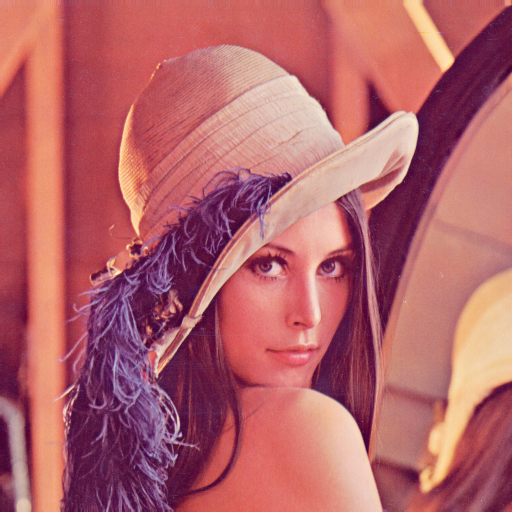
\includegraphics[width=\textwidth]{thesis-template-master/images/lenna.png}
			\caption{Lenna}
			\label{fig:lenna}
		\end{subfigure}
		\begin{subfigure}[b]{0.49\textwidth}
			\reflectbox{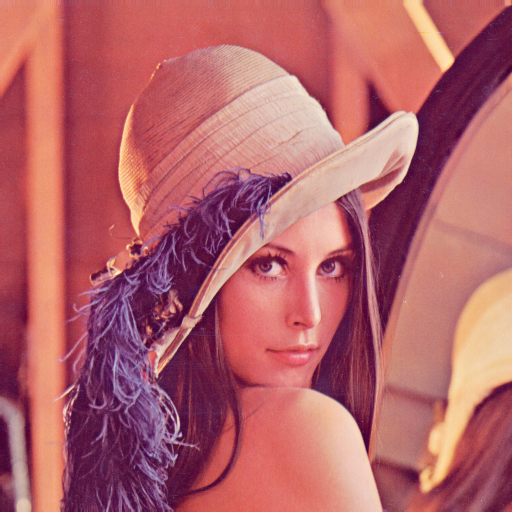
\includegraphics[width=\textwidth]{thesis-template-master/images/lenna.png}}
			\caption{Lenna facing left}
			\label{fig:lenna_facing_left}
		\end{subfigure}
	\end{center}
	\caption{The famous Lenna image used in Computer Vision with subcaptions and a global caption.}
	\label{fig:lennas}
\end{figure}
The figure can be referenced in the text \eg\reffig{lennas}.
Also the subfigures can be referenced \eg\reffig{lenna}, \reffig{lenna_facing_left}.
% subsection figures (end)

\subsection{Citations} % (fold)
\label{sub:citations}
You can cite books from your bibliography \texttt{thesis.bib} (\eg \cite{cochrane}).
Abbreviations from \texttt{abbrev.bib} help in writing the entries.
% subsection citations (end)

\subsection{FixMe warnings}
\label{sub:fixme}
You can add warnings\fxwarning{WARNING} or notifications\fxnote{Note} to your text.
This will help you keep an overview on the places in the text you have to work on.

\section{Lorem}
\label{sec:lorem}


\section{Ipsum}
\label{sec:ipsum}

\subsection{Dolor sit} % (fold)
\label{sub:dolor_sit}


\subsection{Amet} % (fold)
\label{sub:amet}






























\chapter{Methodology}
\label{sec:Methodology}
The purpose of this thesis is to invent a unifying approach that is capable of not only imaging single-cell morphology of thousands of peripheral blood cells, but also data-driven learning of characteristic mythologies indicative of the presence of the disease. With this in mind, we introduce a novel family of deep hierarchical network architectures called AttentionNet. Its goal is to leverage a simple but well-established architecture for nearly-semantic segmentation in order to ensure 
higher precision classification task. Thus, we are able to base our claims about multi-Scale prediction framework and multiple layers concatenation of original YOLOv3 architecture on a variety of experiments individually (see Chapter 5). The idea of this novel AttentionNet architecture is to combine lighter-weight layers  and k-means++ techniques in pre-processing, and GBCIOU multi-object segment techniques such that the network explores and archives the nearly-semantic segmentation for cells with lower cost computation cost and complexity.

For biomedical images processing, due to different experimental conditions, such as lighting condition and various  experimental objects, noise deviations are likely to appear on the sampled cell images\cite{b6}\cite{b7}, those noise and variability in the background would be confounding variables.
When applying attentionnet first, we explicitly learn features focusing on the morphology structure of the object. As we originally designed the unifying approach for Sezary Syndrome, which is an aggressive cutaneous T cell lymphoma that is characterized by presence of tumor T cells with abnormal nucleus morphology in the peripheral blood. Morphological identification of tumor T cells in the blood is currently still the gold standard.
Hence, we assume that after AttentionNet segmentation convolutions are more likely to learn feature representations only for cell objects as only the cell objects are preserved.

Modern architectures leverage multi-scale hierarchies in order to learn feature representations at different resolutions from fine-grained, highly localized features to coarse but semantically enriched features, such as original YOLO network and other state-of-the-art models. On the other hand, it also increases  the complexity of network, requires excessive computational cost and has insufficient sensitivity to customer datasets.

AttentionNet however discards Darknet feature extraction layer of original YOLO, which is a multi convolutional stacked layer, and relies on two yolo output layers. Because the prior of the predicted box is known upfront by k-Mean++ clustering we introduced. Thus, only a few up-sampling layers additional are needed to give a satisfied accurate prediction of the cell position. then, circle detection algorithm will convert Square bounding box to nearly semantic cell prediction while guaranteeing user-defined quality requirements of the cell structure.

Since NMS(Non-Maximum Suppression) of YOLOV3 will only removing prediction boundary boxes that have a high overlap and a low class score, we cannot guarantee good performance in cases such as:multiple cells overlap each other and have high objectiveness scores, or multiple cells do not overlap but are presented in the same frame. It is inevitable to utilize GBCIOU to eliminate objects with relative lower objectiveness score while maximizing retention of overlapping cells.

It is worth noting that the AttentionNet is not involved in the task of cell classification. We therefore introduce CellNet. The main novelty of CellNet is that it creatively combines the features of ResNet\cite{b20} that are easy to expand, easy to understand, and extremely high classification accuracy, and the feature of GhostNet\cite{b19} module that uses a small amount of linear cheap operation to reduce  redundant feature maps, thereby achieving a lighter weight, real-time processing and higher classification accuracy network, especially suitable for the use of complex medical data sets.
%is currently still the gold standard\cite{b3}. There are huge amount of cell images produced from image flow cytometry process, including both healthy data set and diseases data set for comparison. 


\section{AttentionNet}
\label{sec:lorem}


\subsection{Network Architecture} % (fold)
\label{sub:citations}

In Table 3.1, we present our multi-scale AttentionNet architecture which adopts the YOLOV3-Tiny architecture as its fundamental building block in order to process more efficiently on small target. We follow the same
symmetrical encoder-decoder architecture with additional skip-connections interconnected them in the same hierarchy level. At each hierarchy level, we perform several point-wise convolutions in a consecutive manner. 

\begin{table}[h]
\centering

\scalebox{0.90}{
\begin{tabular}{@{}clllll@{}}
\toprule
\multicolumn{1}{l}{\textbf{layer}} & \textbf{Type}                & \multicolumn{1}{l}{\textbf{Filters}} & \textbf{Size/Stride} & \textbf{Input}       & \textbf{Output}                          \\ \midrule
0                                  & Convolutional                & 16                                   & $3\times3$/1       & 416\times416\times3            & 416\times416\times16                               \\
1                                  & Maxpool                      &                                      & $2\times2$/2                & 416\times416\times16           & 208\times208\times16                               \\
2                                  & Convolutional                & 32                                   & $3\times3$/1                & 208\times208\times16           & 208\times208\times32                               \\
3                                  & Maxpool                      &                                      & $2\times2$/2                & 208\times208\times32           & 104\times104\times32                               \\
4                                  & Convolutional                & 64                                   & $3\times3$/1                & 104\times104\times32           & 104\times104\times64                               \\
5                                  & Maxpool                      &                                      & $2\times2$/2                & 104\times104\times64           & 52\times52\times64                                 \\
6                                  & Convolutional                & 128                                  & $3\times3$/1                & 52\times52\times64             & 52\times52\times128                                \\
7                                  & Maxpool                      &                                      & $2\times2$/2                & 52\times52\times128            & 26\times26\times128                                \\
8                                  & Convolutional                & 256                                  & $3\times3$/1                & 26\times26\times128            & 26\times26\times256                                \\
9                                  & Maxpool                      &                                      & $2\times2$/2                & 26\times26\times256            & 13\times13\times256                                \\
10                                 & Convolutional                & 512                                  & $3\times3$/1                & 13\times13\times256            & 13\times13\times512                                \\
11                                 & Maxpool                      &                                      & $2\times2$/1                & 13\times13\times512            & 13\times13\times512                                \\
12                                 & Convolutional                & 1024                                 & $3\times3$/1                & 13\times13\times512            & 13\times13\times1024                               \\
13                                 & Convolutional                & 256                                  & $1\times1$/1                & 13\times13\times1024           & 13\times13\times256                                \\
14                                 & Convolutional                & 512                                  & $3\times3$/1                & 13\times13\times256            & 13\times13\times512                                \\
15                                 & Convolutional                & {\color[HTML]{CB0000} \textbf{18}}   & $1\times1$/1                & 13\times13\times512            & {\color[HTML]{CB0000} \textbf{$13\times13\times18$}} \\
16                                 & YOLO                         &                                      &                      &                      &                                          \\
17                                 & \textbf{Rout13}              &                                      &                      &                      &                                          \\
18                                 & Convolutional                & 128                                  & $1\times1$/1                & 13\times13\times256            & 13\times13\times128                                \\
19                                 & Upsampling                   &                                      & $2\times2$/2                & 13\times13\times256            & 26\times26\times128                                \\
20                                 & \textbf{Route 19, 8}         &                                      &                      &                      &                                          \\
21                                 & Convolutional                & 256                                  & $3\times3$/1                & 26\times26\times384            & 26\times26\times256                                \\
22                                 & Convolutional                & {\color[HTML]{CB0000} \textbf{18}}   & $1\times1$/1                & 26\times26\times256            & {\color[HTML]{CB0000} \textbf{$26\times26\times18$}} \\
23                                 & YOLO                         &                                      &                      &                      &                                          \\ \bottomrule

\end{tabular}}
\caption{\textbf{AttentionNet network structure}. Final YOLO Output should equal to $3\times(classes+5))$}
\end{table}

The attributes of self-detection and labeling, of nearly real-time resolve and of general resource requirements mainly characterize the AttentionNet Network. At the beginning it is  similar to YOLOv3\cite{b33} that the input image is divided into an $M \times M$ grid. Then $B$ bounding boxes and confidence score are defined in each grid cell. Each grid cell predicts $C$ conditional probabilities, denoted as $P(Class_{i}\mid Object_{j})$ for $i$ classes and object $j$. If there is an object $j$ in the grid, then indicated the objectiveness score $P(Object_{j})$  equal to $1$\cite{b18}. Here, we refer the initiatives from YoloV3, the confidence score also represents the accuracy of the box prediction, which is defined as $GIOU_{Ground truth}^{Predition}$. Unlike the originally YOLOv3\cite{b33}, instead of using Intersection‐Over‐Union (IOU), we use $GIOU$ with higher precision, which refers to the generalized intersection area between the predicted bounding box and ground truth box.

It should be noted that each grid cell predicted conditional class probability is not same as the confidence score. These often leads to misunderstanding of the fact that the former $P(Class_{i} \mid Object_{j})$ is predicted in each grid, while the $P(Object_{j}) \times GIOU_{Ground truth}^{Predition}$ is predicted in each bounding box\cite{b18}. 
Finally Class Score $S$ is defined as follow (1): \label{eq}

\begin{equation}
\begin{split}
$S&=P(Class_{i}\mid Object_{j}) \times P(Object_{j}) \times GIOU_{Ground truth}^{Predition} \\
$& = P(Class_{i}) \times GIOU_{Ground truth}^{Predition} $\label{eq}
\end{split}
\end{equation}

The Class Score $S$ computed the probability of the object $j \in  i$ class appearing in the box, as well as how well the bounding box fits each object $j$.






\subsection{Multi Scale Tensor Prediction Framework}
\label{sub:fixme}

The original YOLOv3\cite{b33} used the darknet front-end feature extraction module, but the detection performance on Sezary Syndrom dataset is unsatisfied. On the contrary, AttentionNet with only $13 \times 13$, $26 \times 26$ yolo scale output tensors adopts multi-scale fusion, and K means++ clustering\cite{b18} techniques, outperforms TF-Yolo\cite{b18} and  YOLOv3 \cite{b33}, which has $13 \times 13$, $26 \times 26$, $52 \times 52$ yolo scale output tensor. In order to train a suitable segment-or, it is recommended to choose corresponding scale tensors refer to different data sets. 

We use a YOLOV3 like architecture due to its modularisation capabilities. In the ablation study, we individually measure the impact of all architectural components. Here, we vary the tensor Multi Scale Tensor, as well as the number of hierarchy levels used by the architecture. Moreover, we vary the number of point-wise convolution layers to measure the effect of each Yolo tensor output independently and in parallel. Hence, we make reasonable
claims about the combination of only $13 \times 13$, $26 \times 26$ yolo scale output tensors.

\begin{figure}[h]
	\begin{center}
		\begin{subfigure}[b]{0.49\textwidth}
			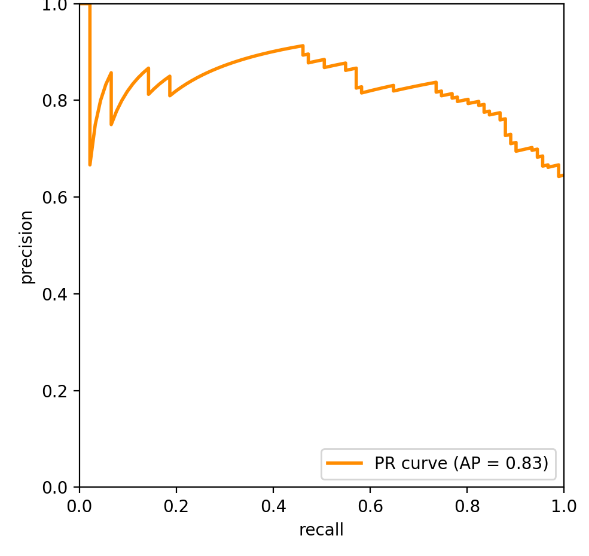
\includegraphics[width=\textwidth]{thesis-template-master/images/2 tensor cellyolo PR on val dataset.png}
			\caption{$13 \times 13$, $26 \times 26$ tensor Cellyolo PR on val dataset}
			\label{fig:res18}
		\end{subfigure}
		\begin{subfigure}[b]{0.49\textwidth}
		    \centering
			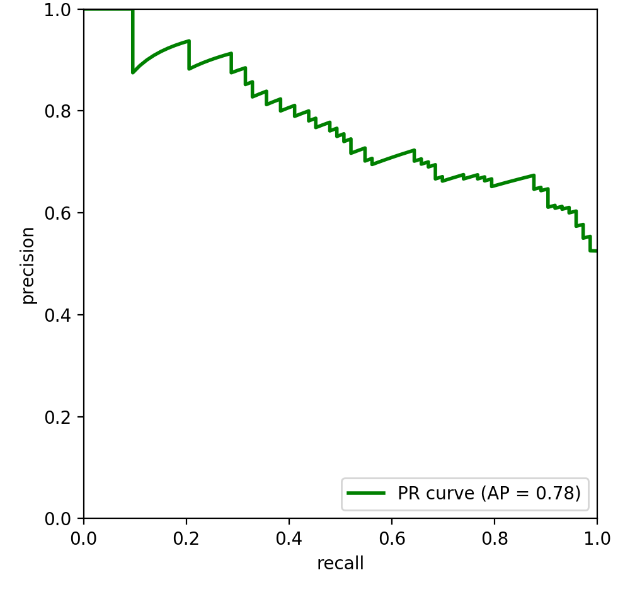
\includegraphics[width=\textwidth]{thesis-template-master/images/52 tensor cellyolo PR on val dataset.png}
			\caption{$52 \times 52$, $26 \times 26$tensor Cellyolo PR on val dataset}
			\label{fig:cellnet}
		\end{subfigure}
	\end{center}
	\caption{Precision-Recall curve on val sub-dataset of Sezary Syndrom dataset (1k training image, 726 test image), in terms of different scale yolo output layers}
\end{figure}



\subsection{K‐means++ Clustering in Pre-processing}

K‐means++ clustering is an approach commonly used to adaptive partition a dataset into groups. It is necessary to specify the number of cluster centers in advance. The k‐means++ algorithm generally uses the Euclidean distance to measure the distance between two points. Instead of using prior 9 box given by YOLOv3 trained on COCO dataset, for our customer dataset, it's noteworthy that give the prior knowledge of ground truth box. Using small subset of manually annotated cell, we can improve $GIOU$(ground truth box position, prediction box location) scores, and these will leads to better class scores as well and in final achieve higher accuracy.

\begin{figure}[h]
	\begin{center}
		\begin{subfigure}[b]{0.49\textwidth}
			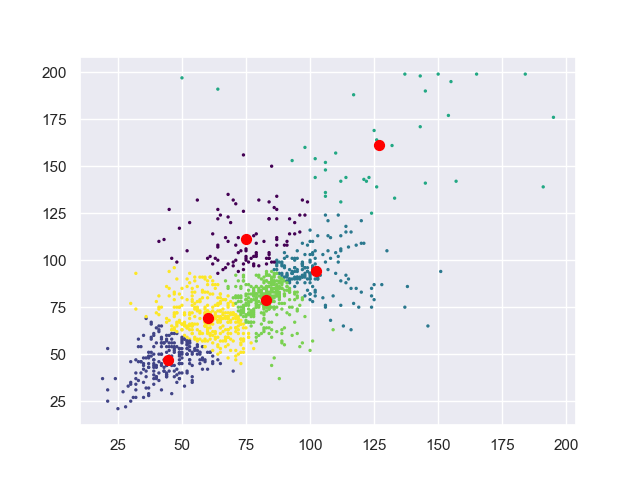
\includegraphics[width=\textwidth]{thesis-template-master/images/Figurefor 1480_1.png}
			\caption{ Six prior boxs}
			\label{fig:res18}
		\end{subfigure}
		\begin{subfigure}[b]{0.49\textwidth}
		    \centering
			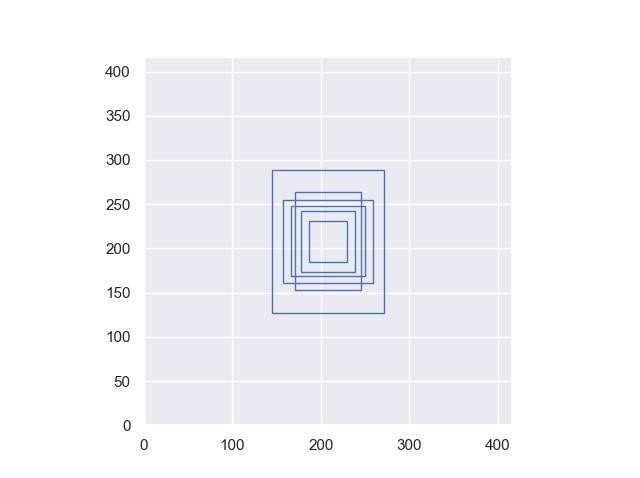
\includegraphics[width=\textwidth]{thesis-template-master/images/Figure_for1480.png}
			\caption{The cluster distribution}
			\label{fig:cellnet}
		\end{subfigure}
		\begin{subfigure}[b]{0.49\textwidth}
			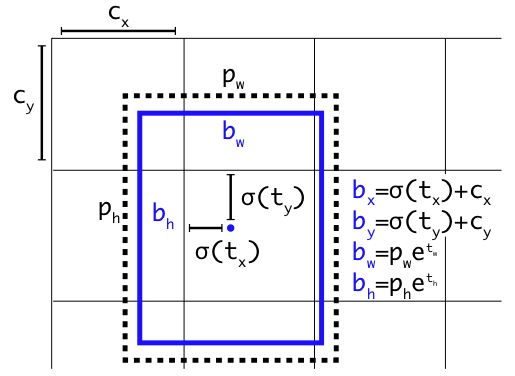
\includegraphics[width=\textwidth]{thesis-template-master/images/anchor.JPG}
			\caption{ Prior box and location prediction box}
			\label{fig:res18}
		\end{subfigure}
	\end{center}
	\caption{\textbf{The comparison between normal convolutional layer in \cite{b26}\cite{b27}\cite{b28} and ghost module}. We only take point-wise convolution once to get a few intrinsic feature maps, then we utilized the linear cheap transformation to generate ghost map with lower cost.}
\end{figure}

Nevertheless, there are the following three scale targets in the dataset: large‐scale targets, moderate‐scale targets, and small‐scale targets [30]. The main steps of the K‐means++ method are as follows:  The definition of the three sizes of targets here refers to the proportion that they are in the entire image.
\begin{figure}[h]
	\begin{center}
		\begin{subfigure}[b]{0.49\textwidth}
		    \centering
			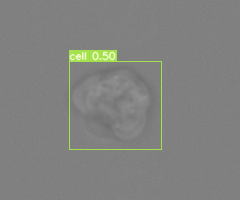
\includegraphics[width=0.9\textwidth]{thesis-template-master/images/withkmean.png}
			\caption{With k-means++ cluster}
			\label{fig:cellnet}
		\end{subfigure}
		\begin{subfigure}[b]{0.49\textwidth}
		    \centering
			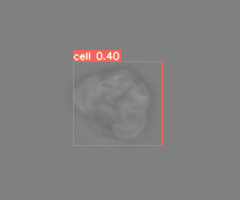
\includegraphics[width=0.9\textwidth]{thesis-template-master/images/withoutkmean.png}
			\caption{Without k-means++ cluster}
			\label{fig:cellnet}
		\end{subfigure}
		\begin{subfigure}[b]{0.49\textwidth}
		    \centering
			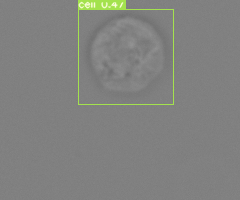
\includegraphics[width=0.9\textwidth]{thesis-template-master/images/withkmean1.png}
			\caption{With k-means++ cluster}
			\label{fig:cellnet}
		\end{subfigure}
		\begin{subfigure}[b]{0.49\textwidth}
		    \centering
			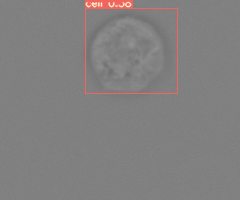
\includegraphics[width=0.9\textwidth]{thesis-template-master/images/withoutkmean2.png}
			\caption{Without k-means++ cluster}
			\label{fig:cellnet}
		\end{subfigure}
	\end{center}
	\caption{\textbf{The comparison between normal convolutional layer in \cite{b26}\cite{b27}\cite{b28} and ghost module}. We only take point-wise convolution once to get a few intrinsic feature maps, then we utilized the linear cheap transformation to generate ghost map with lower cost.}
\end{figure}


\begin{algorithm}[h]
  \caption{K‐means++ Clustering in ground truth boxes.}
  \label{alg:Framwork}
  \begin{algorithmic}[1]
    \Require
    manually labelled a series of ground truth $B^{i}$ bounding boxes coordinates:
     $B^{i}=\left ( x_{1}^{i},y_{1}^{i},x_{2}^{i},y_{2}^{i} \right ), i\in n.$ And clusters number $K$
    \Ensure
    optimal  prediction box size $\left ( w,h \right )$
    \State For each box $B^{i}$, calculated the width and height by:
    
    $w^{i}=(x_{2}^{i}-x_{1}^{i}), h^{i}=(x_{2}^{i}-x_{1}^{i})$, 
    
    \State Choose an initial center $t_{1}$ uniformly at random from the dataset $X=(w^{i},h^{i}),i\in n$.
    \While{$d\left ( x \right )$ shortest distance and  $K$ cluster not reached}
       \State Choose the next center $t_{i}$ , selecting $t_{i}={x}'\in X $ with probability $\frac{d ( {x}')^{2}}{\sum_{x\in X}^{}d\left ( x \right )^{2} }$
where $d\left ( x \right )$ is the distance from a data point $x$ to the closest cluster center.
       \State For $i \in \left \{ 1,2,...K \right \}$ , set the cluster $T_{i}$ to be the set of points in $X$ that are closer to
$t_{i}$ than they are to $t_{j}$ for all $i\neq j$.
    
  
    \Return $T_{i}=(w^{i},h^{i}),i \in K$.
  \end{algorithmic}
\end{algorithm}

As mentioned above, YOLOv3 algorithm has achieved end‐to‐end training and high‐speed target detection. However, some problems still exist. Conventional YOLO divides each image into a fixed grid, which results in the number of detected objects will be limited. The fixed parameters provided by anchor are suitable for the targets in the VOC datasets, while they are not adapted to the targets in specific scenes. Common targets, such as vehicles, tanks, and airplanes, have a large aspect ratio. Therefore, this section takes advantage of the ideas in Fast R‐CNN and SSD to re‐cluster according to a spacific scenario. In the beginning, the network manually sets a priori box. To guarantees the selection of network is more subjective, and it would make the deep network easier to learn. Furthermore, its predictions perform better than the original method. In order to optimize the adapted parameters and select appropriate anchor box size, the designed network needs to recluster according to real application domains. In this way, the AttentionNet network achieve nearly semantic prediction, meanwhile, it is insensitive to small objects particularly.




\subsection{Loss function} % (fold)
\label{sub:citations}

Contrarily to the original implementation of YOLOv3 (Chapter 2.3.2), we calculate the loss function by means of three parts. Here, we divide them into three compositions, the loss between the ground truth box and the prediction box, the confidence score loss, the final cross entropy loss for class label. First part is the prediction bounding box loss, second part indicates the confidence loss and final part represents the class label loss. k means the classes, the conf states the confidence, and the 10647 generated from 2535 prediction bounding boxes. It is equal to $(13\times13\time3+26\time26\time3)=2535$ in contrast to originally YOLOv3 has $(13\times13\time3+26\time26\time3+26\time26\time3)=10647$ prediction bounding boxes.

\begin{equation}
\begin{split}
$Loss&=\frac{1}{2}\sum_{i=1}^{2535}\lambda _{obj}\times \{ \left ( 2-truth_{w} \times truth_{h}\right )\times  \sum_{r\in \left ( x,y,w,h \right )}^{}\left ( truth_{r}-predict_{r} \right )^{2} \\$
$&+ \sum_{k-1}^{r=0} \left ( \left ( r==truth_{class} \right )-predict_{class_{r}} \right )^{2}  \} + \left ( truth _{conf}-predict_{conf}\right )^{2}$\label{eq}
\end{split}
\end{equation}


\textbf{ The Loss for Bounding Box}:
\begin{equation}
\begin{split}
$\lambda _{obj}\times \left  \left ( 2-truth_{w} \times truth_{h}\right )\times \sum_{r\in \left ( x,y,w,h \right )}^{}\left ( truth_{r}-predict_{r} \right )^{2}$ \label{eq}
\end{split}
\end{equation}
In YOLOv1, the author did find the square root of the width and height (w, h), in order to Weakening the influence of the bounding box size on the loss value. Here, we are following YOLOv3 priority suggestions do not adopt the square root method, but added a weight related to the size of the  object box size. namely with weight = $  2-truth_{w} \times truth_{h}  $, value range from (1~2). In contrast to the first version of YOLO network, which adopted the IOU loss to calculate the loss between  prediction box and prior, the YOLOv3 imporved the accuracy by 1\% under the  contribution of GIOU loss. 

\begin{algorithm}[htb]
  \caption{ Generalized Intersection over Union(GIoU) as Bounding Box loss.}
  \label{alg:Framwork}
  \begin{algorithmic}[1]
    \Require
    Predicted $B^{p}$ and ground truth $B^{g}$ bounding box coordinates:
     $ B^{p}=\left ( x_{1}^{p},y_{1}^{p},x_{2}^{p},y_{2}^{p} \right ),B^{g}=\left ( x_{1}^{g},y_{1}^{g},x_{2}^{g},y_{2}^{g} \right ).$
    \Ensure
     GIoU loss $L_{GIoU}$;
    \State For the predicted box $B^{p}$, ensuring $x_{2}^{p} > x_{1}^{p}$ and $y_{2}^{p} > y_{1}^{p}$:
    
    $\hat{x}_{1}^{p}=min( x_{1}^{p},x_{2}^{p})$, $\hat{y}_{1}^{p}=min( y_{1}^{p},y_{2}^{p})$,
    $\hat{x}_{2}^{p}=max( x_{1}^{p},x_{2}^{p})$, $\hat{y}_{2}^{p}=max( y_{1}^{p},y_{2}^{p})$.

    
    \State Calculating the area of $B^{g}$:
    $A^{g}=(x_{2}^{g}-x_{1}^{g}) \times (y_{2}^{g}-y_{1}^{g})$
   
    \State  Calculating the area of $B^{p}$:
    $A^{p}=(\hat{x}_{2}^{p}-\hat{x}_{1}^{g}) \times (\hat{y}_{2}^{p}-\hat{y}_{1}^{p})$
    
    \State Calculating the intersection area $I$ between  $B^{g}$and  $B^{p}$:
    
    $x_{1}^{I}=max( \hat{x}_{1}^{p},x_{1}^{g})$, $y_{1}^{p}=max( \hat{y}_{1}^{p},y_{1}^{g})$,
    $x_{2}^{I}=min(\hat{x}_{2}^{p},x_{2}^{g})$, $y_{2}^{p}=min(\hat{y}_{2}^{p},y_{2}^{g})$.
    \If {$x_{1}^{I} < x_{2}^{I},  y_{1}^{I} < y_{2}^{I} $}
      \State  $I= (x_{2}^{I}-x_{1}^{I}) \times (y_{2}^{I}-y_{1}^{I})$ 
    \Else
      \State $I \gets 0$
      
    \EndIf
    \State Finding the coordinate of the smallest enclosing convex object $C$:
      $ C=\left ( min( \hat{x}_{1}^{p},x_{1}^{g}), max(\hat{x}_{2}^{p},x_{2}^{g}),
      min( \hat{y}_{1}^{p},y_{1}^{g}), max(\hat{y}_{2}^{p},y_{2}^{g}) \right )$
    
    \State Calculating area of the smallest enclosing convex object $S^{C}$
    \State $IoU=I/( A^{g} + A^{p} - I)$
    \State $GIoU=  IoU -\frac{S^{C}-A^{g} - A^{p} + I}{S^{C}}$
    \State $L_{GIoU}=1-GIoU$
    
    \Return $L_{GIoU}$.
  \end{algorithmic}
\end{algorithm}

In cvpr2019 paper GIOU, they proposed a new way to optimize boundary boxes mode, defined as generalized IOU, the bounding box is generally composed of the upper left and lower right corners of the coordinates, denoted as (x, y, x2, y2). Note that this is actually a vector, and vector distances are generally can be measured by either the L1 norm or the L2 norm.

However, when either the L1 or L2 norms is the same, it was found that the values of both IOU and GIOU are very different, indicating that the use of the L paradigm to measure the the distance between  the prediction and the real ground truth is inappropriate.



\begin{figure}[h]
	\begin{center}
		\begin{subfigure}[b]{0.49\textwidth}
		    \centering
			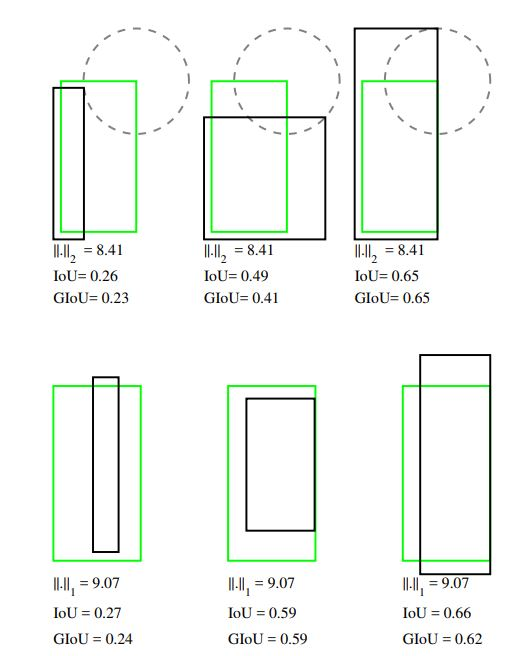
\includegraphics[width=\textwidth]{thesis-template-master/images/l2loss.JPG}
			\label{fig:cellnet}
		\end{subfigure}
	\end{center}
	\caption{Two sets of examples with the bounding
boxes represented by two corners (x1, y1, x2, y2) for first row, center and size (xc, yc, w, h) for second row. For all three cases in each set$ ℓ2$
norm distance, and  $ℓ1$-norm distance, between the representation of two rectangles are exactly same value, but their IoU and GIoU values are very different.}
\end{figure}


In this case, the IOU is commonly used in academia to measure the similarity between two boundaries, but we found experimentally that there are two obvious drawbacks to using IOU which makes it less suitable for the loss function.

First, when there is no overlap between the prediction box and the ground truth. An IOU value of 0 results in a gradient of 0 when optimizing the loss function, meaning that optimization is not possible.

secondly, even if the prediction box and the real box overlap and have the same IOU value, the detection effect will be very different. This is indistinguishable by IOU, because IOU is the same, but this can be reflected by GIOU . If the two bounding boxes overlap the better, the better the alignment, the higher the GIOU value.

\textbf{ The confidence score loss}:
\begin{equation}
\begin{split}
$\left ( truth _{conf}-predict_{conf}\right )^{2}$ \label{eq}
\end{split}
\caption{\textbf{The Loss for Bounding Box}.}
\end{equation}


First, we should find the prediction bounding box with the largest IOU value of the real ground truth. If the largest IOU is less than the threshold, then the prediction is considered to contain no objects, and it is the background grid. Then we calculate the   confidence loss (we hope that if the grid contains objects, then the confidence of the prediction box output is 1, and 0 when there is no object). The confidence $\lambda _{obj}$ comes from focal loss. It indicates the confidence level to determine if there is an object in the grid.

\textbf{ The cross entropy loss for class label:}
\begin{equation}
\begin{split}
$\lambda _{obj}\times \sum_{k-1}^{r=0}  ( ( r==truth_{class}  )-predict_{class_{r}} )^{2} $ \label{eq}
\end{split}
\caption{\textbf{The Loss for Bounding Box}.}
\end{equation}
Finally,we  utilize the cross entropy loss to generate the class label.


\subsection{GBCIOU and Circle segmentation}
\label{sub:fixme}



\begin{algorithm}[htb]
  \caption{ GBCIOU for objects overlapping}
  \label{alg:Framwork}
  \begin{algorithmic}[1]
    \Require
     Two cell object Prediction $A$ and $B$ bounding box coordinates in the same flame:
     $ B=\left ( x_{1}^{b},y_{1}^{b},x_{2}^{b},y_{2}^{b} \right ),A=\left ( x_{1}^{a},y_{1}^{a},x_{2}^{a},y_{2}^{a} \right ).$ And confidence Score of each object $S^{b}>S^{a}$.
    \Ensure
     Optimal prediction box $P$. 
    \State For the box $A$ and $B$, ensuring: $x_{2}^{b} > x_{1}^{b}$, $y_{2}^{b} > y_{1}^{b}$, $x_{2}^{a} > x_{1}^{a}$, $y_{2}^{a} > y_{1}^{a}$.
    \State Calculate the intersection area:
    
    $I= (min(x_{2}^{a}, x_{2}^{b}) - max(x_{1}^{a}, x_{1}^{b})) \times (min(y_{2}^{a},y_{2}^{b})- max(y_{1}^{a},y_{1}^{b})) $
    \State Calculating the Union area, contrarily to the original Union we add small $1e-16 $
    to balance the integral side effect of $A$ and $B$ bounding box coordinates, but it will not effect the $GIoU$: 
    $Union= (x_{2}^{b}-x_{1}^{b}) \times (y_{2}^{b}-y_{1}^{b})+ 1e-16 + (x_{2}^{a}-x_{1}^{a}) \times (y_{2}^{a}-y_{1}^{a}) -I $
    \State Finding the coordinate of the smallest enclosing convex object $C_{w,h}$: 
    
    $ w, h= max(x_{2}^{a}, x_{2}^{b}) - max(x_{1}^{a}, x_{1}^{b}), max(y_{2}^{a},y_{2}^{b}) - max(y_{1}^{a}, y_{1}^{b})$
    \State Calculating  enclose area  $E$: $E = w \times h + 1e-16$
    \State Calculating  $GIoU$: $GIoU= \frac{E - Union}{E}$ 
    \If { $GIoU < threshold $}
      \State  $P \gets( min(x_{1}^{a}, x_{1}^{b}), min(y_{1}^{a},y_{1}^{b}),max(x_{2}^{a}, x_{2}^{b}),max(y_{2}^{a},y_{2}^{b})) $ 
    \Else
      \State $P \gets (x_{1}^{b},y_{1}^{b},x_{2}^{b},y_{2}^{b})$
    \EndIf
    
    \Return $P$
    
  \end{algorithmic}
\end{algorithm}




\begin{figure}[h]
	\begin{center}
		\begin{subfigure}[b]{0.25\textwidth}
		    \centering
			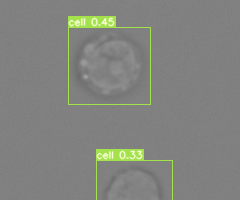
\includegraphics[width=\textwidth]{thesis-template-master/images/gbciou1.png}
			\caption{}
			\label{fig:cellnet}
		\end{subfigure}
		\begin{subfigure}[b]{0.25\textwidth}
		    \centering
			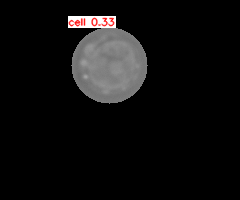
\includegraphics[width=\textwidth]{thesis-template-master/images/gbciou2.png}
			\caption{}
			\label{fig:cellnet}
		\end{subfigure}
		\begin{subfigure}[b]{0.25\textwidth}
		    \centering
			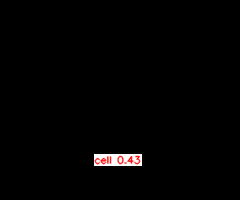
\includegraphics[width=\textwidth]{thesis-template-master/images/gbciou3.png}
			\caption{}
			\label{fig:cellnet}
		\end{subfigure}
		\begin{subfigure}[b]{0.25\textwidth}
		    \centering
			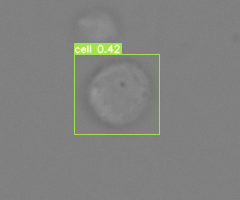
\includegraphics[width=\textwidth]{thesis-template-master/images/gbciou7.png}
			\caption{}
			\label{fig:cellnet}
		\end{subfigure}
		\begin{subfigure}[b]{0.25\textwidth}
		    \centering
			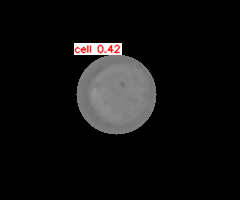
\includegraphics[width=\textwidth]{thesis-template-master/images/gbciou8.png}
			\caption{}
			\label{fig:cellnet}
		\end{subfigure}
		\begin{subfigure}[b]{0.25\textwidth}
		    \centering
			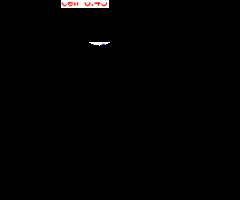
\includegraphics[width=\textwidth]{thesis-template-master/images/gbciou9.png}
			\caption{}
			\label{fig:cellnet}
		\end{subfigure}
		\begin{subfigure}[b]{0.25\textwidth}
		    \centering
			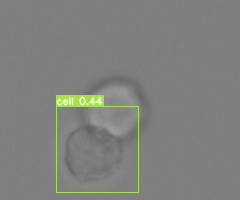
\includegraphics[width=\textwidth]{thesis-template-master/images/gbciou10.png}
			\caption{}
			\label{fig:cellnet}
		\end{subfigure}
		\begin{subfigure}[b]{0.25\textwidth}
		    \centering
			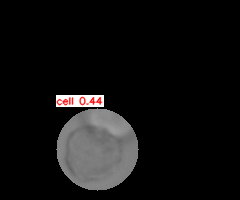
\includegraphics[width=\textwidth]{thesis-template-master/images/gbciou11.png}
			\caption{}
			\label{fig:cellnet}
		\end{subfigure}
		\begin{subfigure}[b]{0.25\textwidth}
		    \centering
			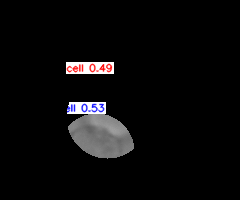
\includegraphics[width=\textwidth]{thesis-template-master/images/gbciou12.png}
			\caption{}
			\label{fig:cellnet}
		\end{subfigure}
	\end{center}
	\caption{\textbf{Experiments on GBCIOU for multiple predictions occur in same cell images}}
\end{figure}

Using the cvfillPoly function, we can easily classify the cell image into simple polygonal areas and achieve high-speed segmentation once we obtain the output from AttentionNet network for anchor box detection, namely ( $x_{1}$, $y_{1}$, $x_{2}$, $y_{2}$). However, it has very obvious shortcomings that the shape of the segmentation does not perfectly approximate the ground truth of the cell. To overcome this problem, we proposed $HSV$ space mask threshold method, simply converting to $HSV$ space and using threshold to eliminate the outside part of central circle of box detection.  For the common challenge of the YOLO original version: when multiple objects standing in the same area or overlapping in the central point, it will become much more difficult to draw the correct prediction and always leads to wrong labeling. In our case if multiple cells occur and one cell has more competitive confidence score than another during circle detection that will leads to either non-labelled or partly labelled problem.

We proposed the GBCIOU function to ideally find general intersected box center when multiple box predictions occur in the same image, in addition to the GIOU (general interaction of union) computes the deviation between ground truth and the prediction.

\section{CellNet}
\label{sec:ipsum}


\subsection{Network Architecture} % (fold)
\label{sub:Network Architecture_2}
Inspired by those two outstanding neural network\cite{b19}\cite{b20}, instead of stacking lots of point-wise convolutional layers and taking huge amount of convolutional manipulations, we can avoid the redundant feature maps by cheap operation. 
%Especially, the only interest of the regions after taking AttentionNet pre-processing will focus on the cell as all the artifacts existed on the images have already been eliminated.

As shown in Table 1. The first layer of CellNet is a standard convolutional layer with 64 filters, follows standard batch normalization and relu, in order to generate initial intrinsic feature maps, then we purpose a few series of G-bneck, namely 8 layers. In each stage first apply stride = 1 then apply stride = 2 bottleneck which gradually increase the output channel dimension. After 8 layer feature extraction, we get a 512-dimensional feature vector by global average pooling and convolutional layer. SE layer applied to scale less important feature map. Smoothing, blurring and motion are also widely used linear operation, but they need more GPU support. By using depth-wise convolution layer, we can generate more correlated ghost feature maps with cheaper cost.



\begin{figure}[h]
	\begin{center}
		\begin{subfigure}[t]{0.49\textwidth}
		    \centering
			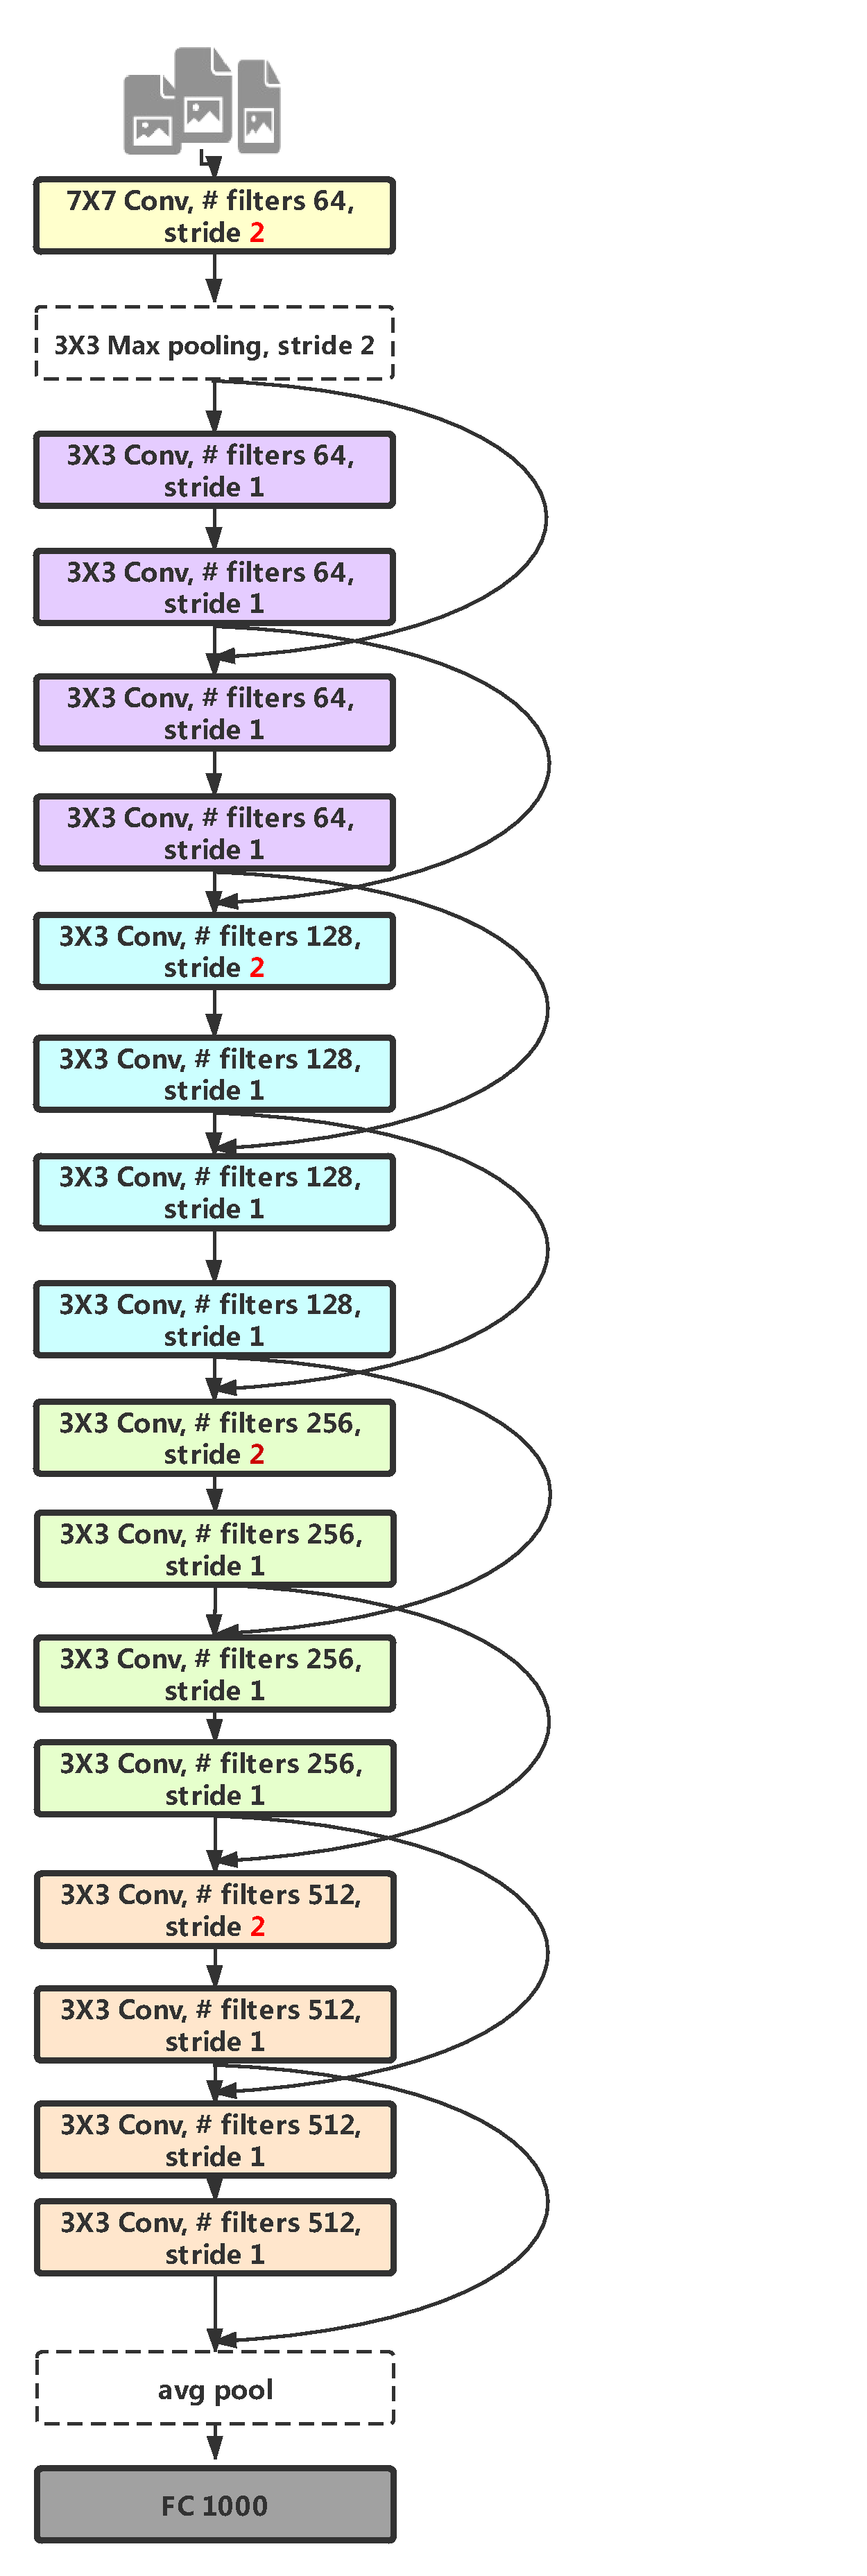
\includegraphics[height=6in]{thesis-template-master/images/res18.pdf}
			\caption{Overall architecture of ResNet18}
			\label{fig:res18}
		\end{subfigure}
		\begin{subfigure}[t]{0.49\textwidth}
		    \centering
			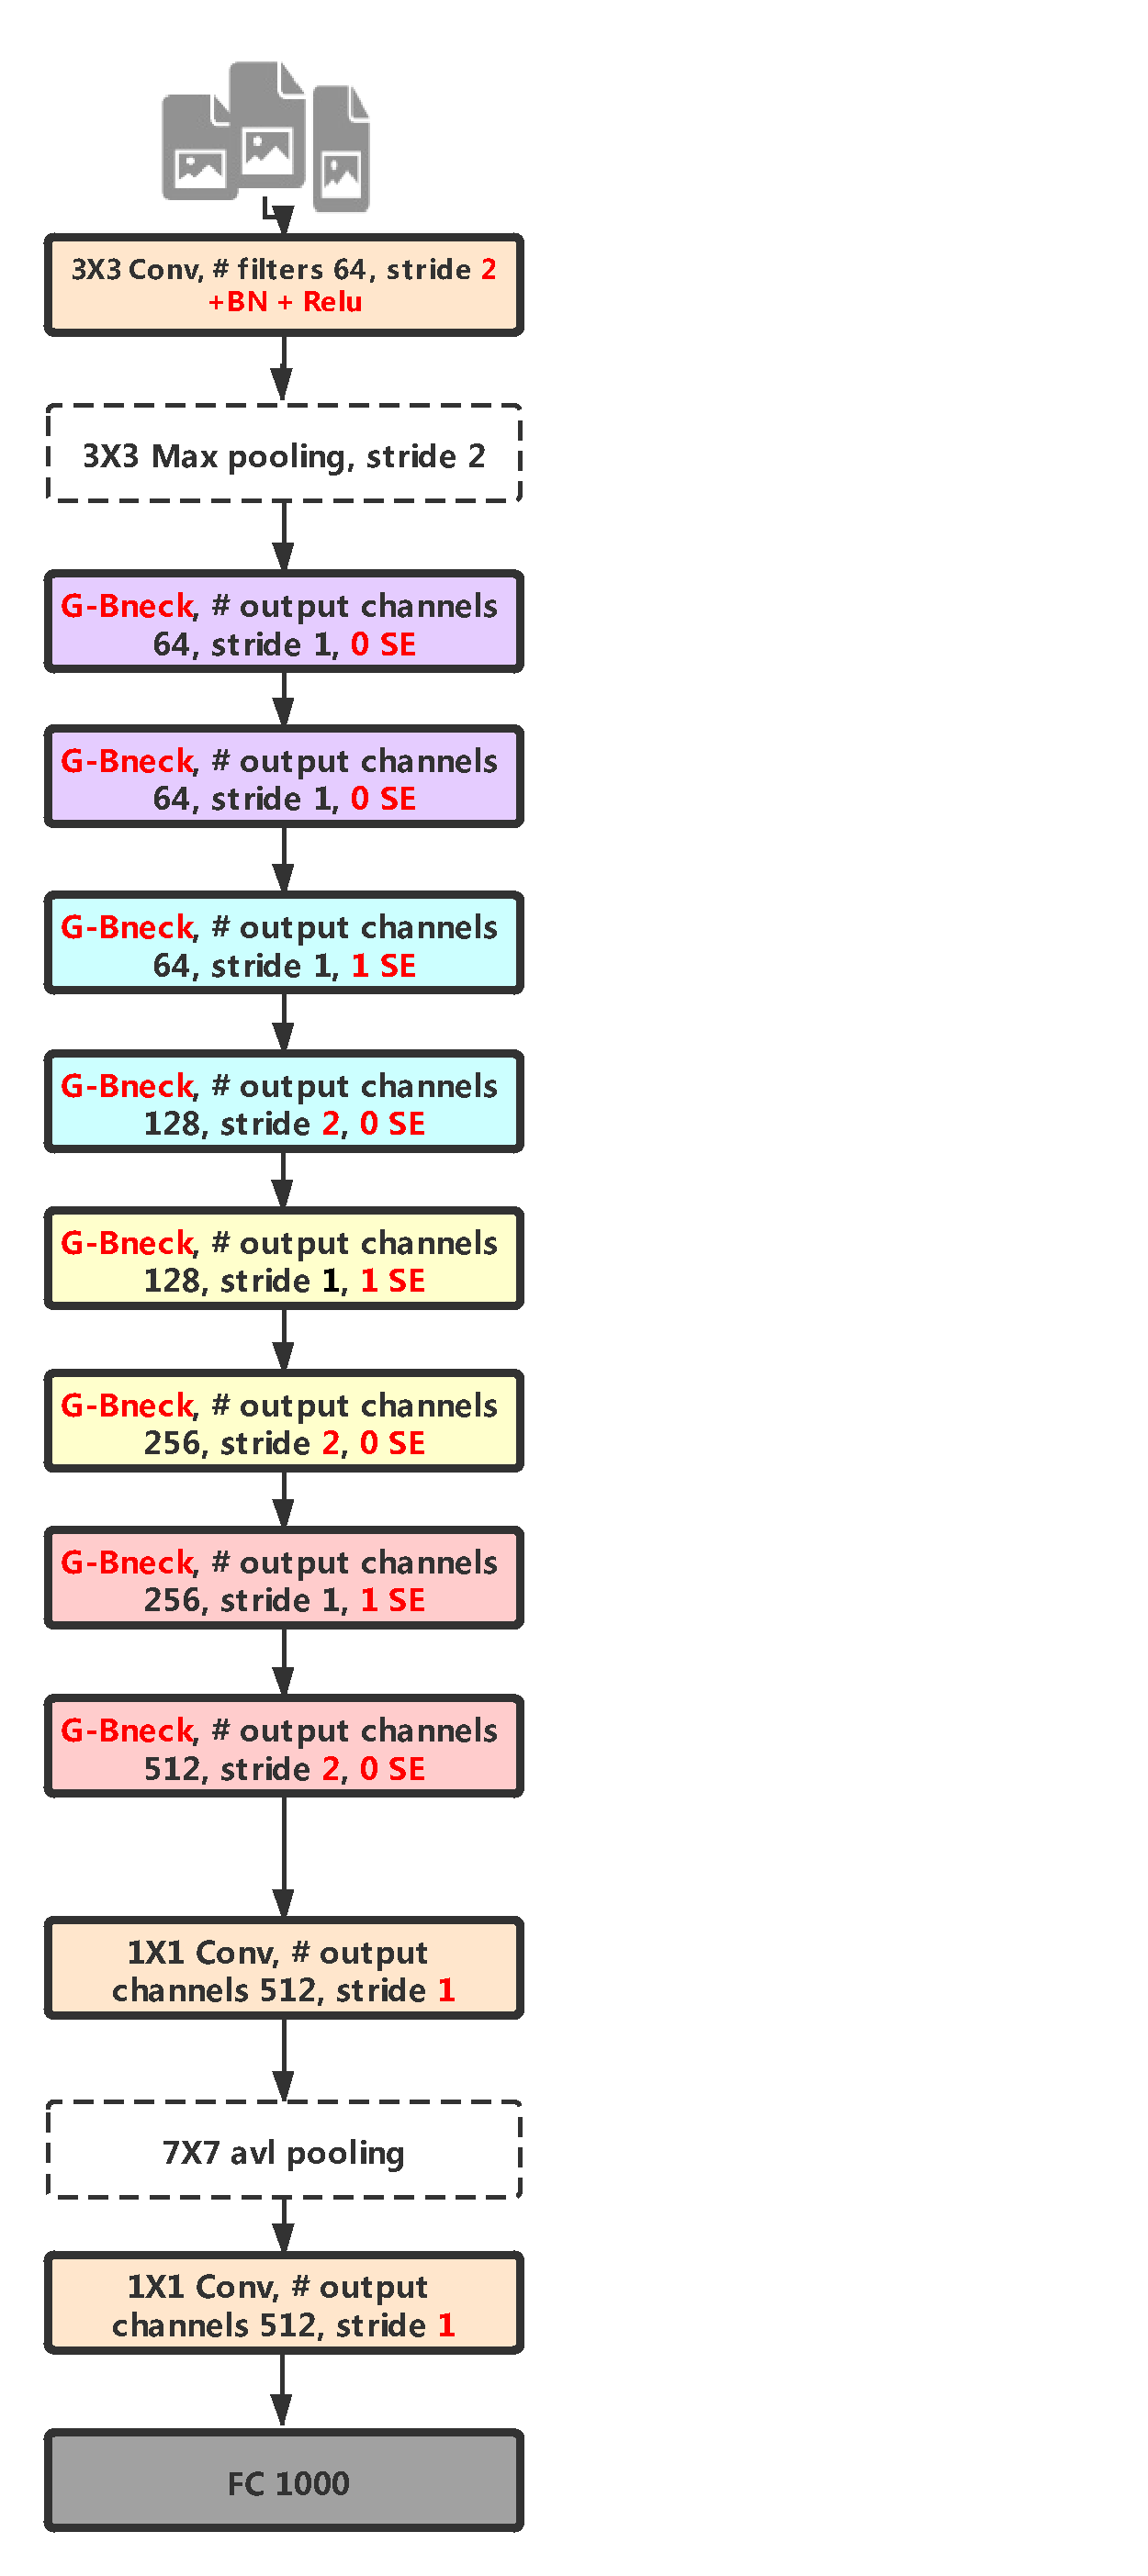
\includegraphics[height =5in]{thesis-template-master/images/Ghostres18.pdf}
			\caption{Overall architecture of CellNet}
			\label{fig:cellnet}
		\end{subfigure}
	\end{center}
	\caption{\textbf{The comparison between ResNet18 \cite{b20} and CellNet}. Despite its simplicity (only 8 layers ghost module) and lower parameters ( $1/4$ weights than ResNet18 \cite{b20}), inside Ghost bottleneck adopted residual function for deeper gradient forward.}
\end{figure}








\subsection{Novel Ghostmodule} % (fold)
\label{sub:amet}

\begin{figure}[h]
	\begin{center}
		\begin{subfigure}[b]{\textwidth}
		    \centering
			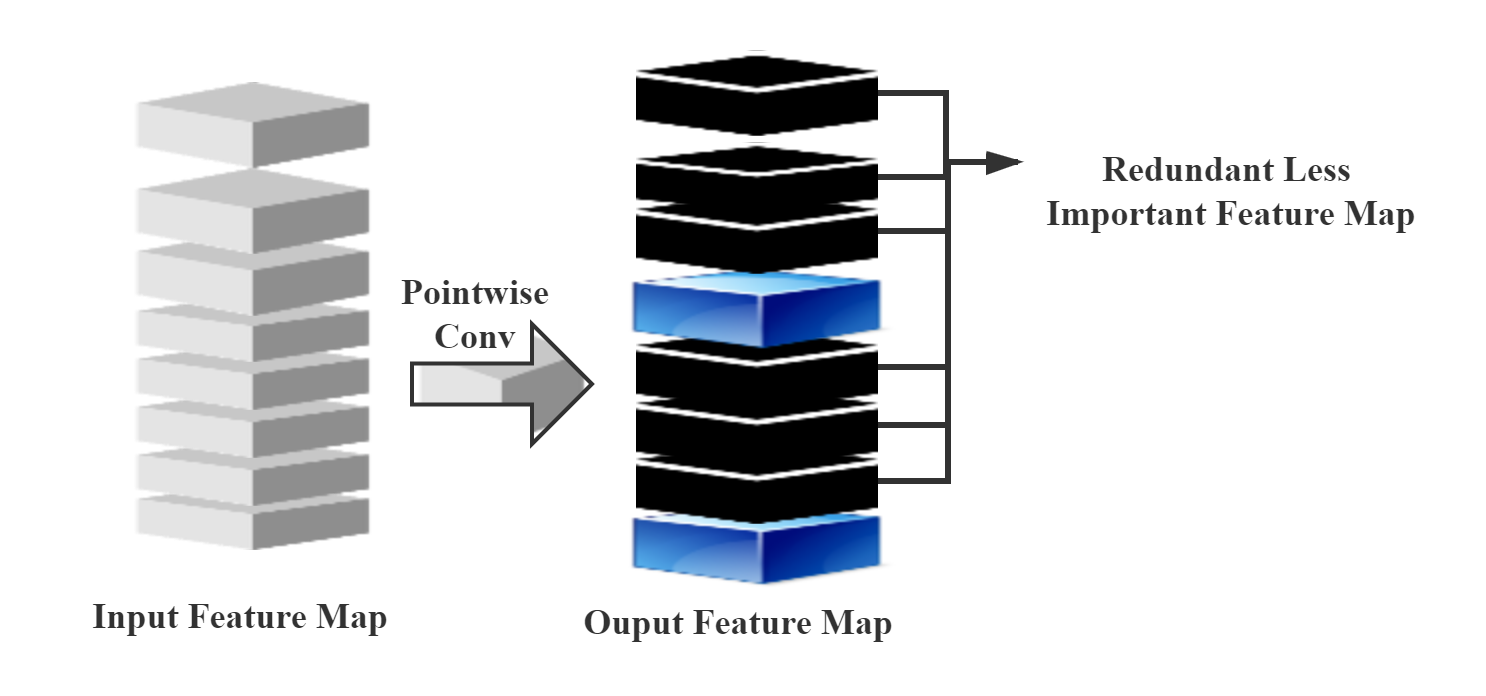
\includegraphics[width=\textwidth]{thesis-template-master/images/normal conv.png}
			
			\label{fig:cellnet}
		\end{subfigure}
	\end{center}
	\caption{\textbf{The normal Convolutional layer in \cite{b26}\cite{b27}\cite{b28}}. As its illustrated that to extraction the same amount of feature map, there are much more redundant output feature map by taking point wise convolution, especially for the small target objects or less informative images.}
\end{figure}


\begin{figure}[h]
	\begin{center}
		
		\begin{subfigure}[b]{\textwidth}
		    \centering
			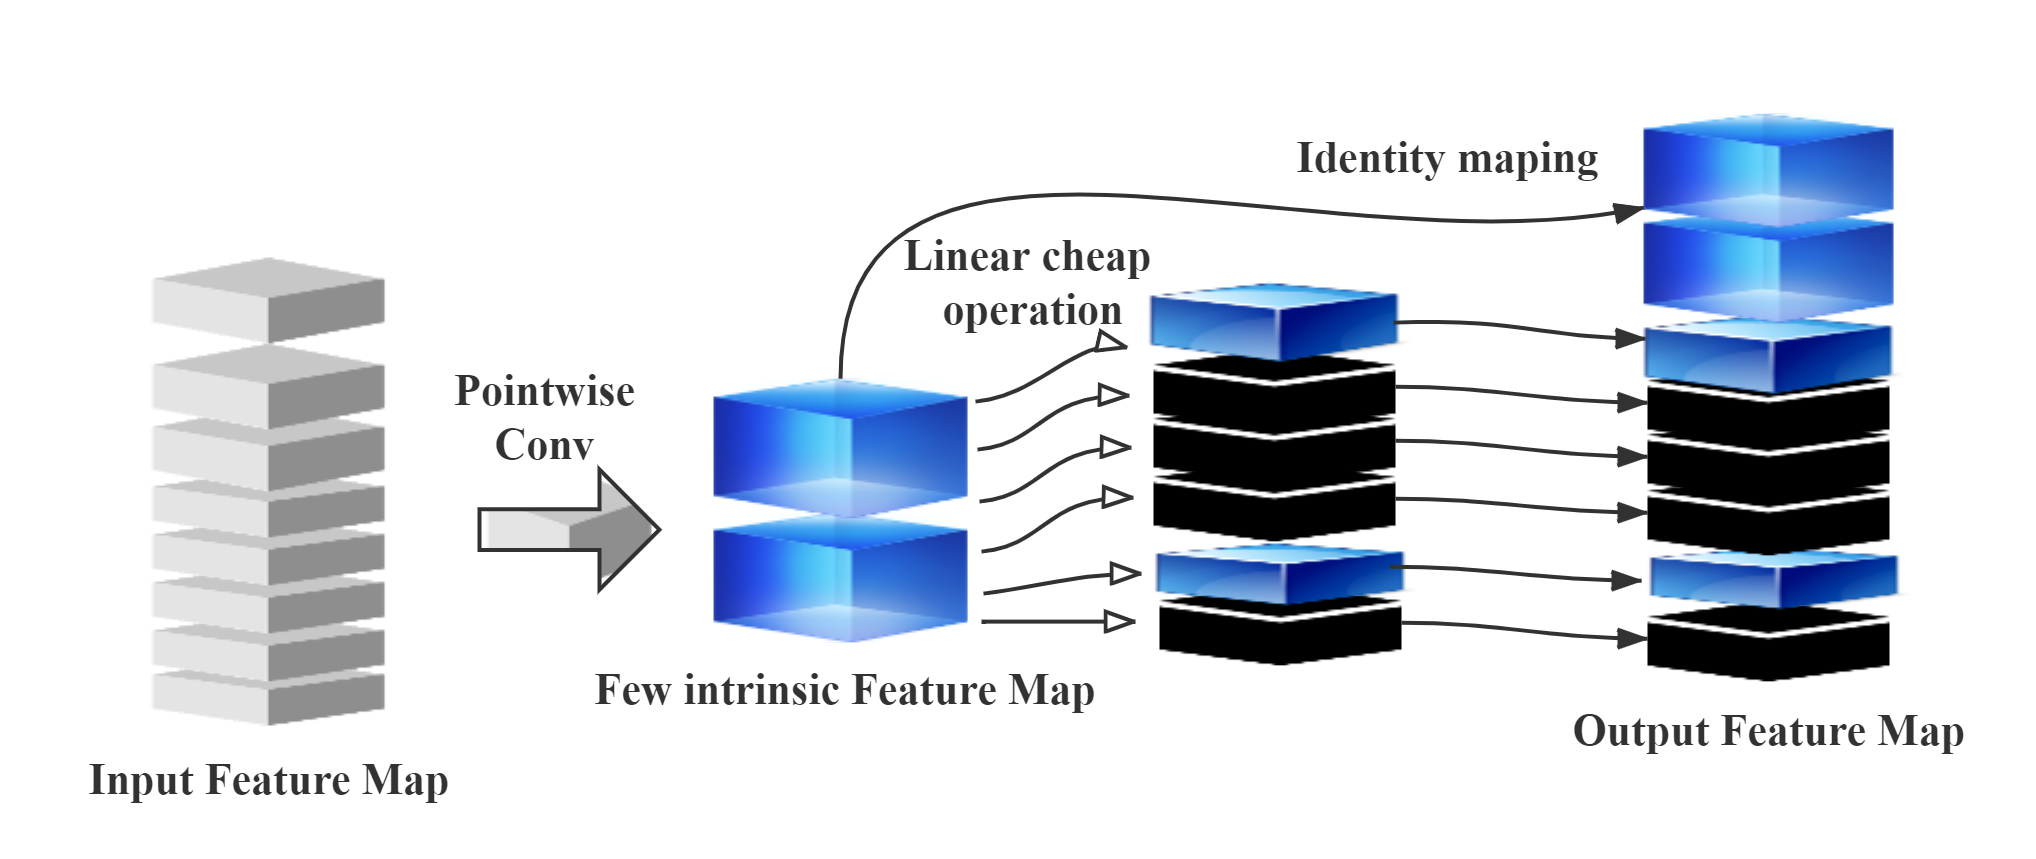
\includegraphics[width=\textwidth]{thesis-template-master/images/ghostmodule.png}
			
			\label{fig:cellnet}
		\end{subfigure}
	\end{center}
	\caption{\textbf{The ghost module layer in \cite{b19}}. We only take point-wise convolution once to get a few intrinsic feature maps, then we utilized the linear cheap transformation to generate ghost map with lower cost.}
\end{figure}

Unlike Ghost module applied in GhostNet\cite{b19}, we designed two kind of novel Ghost Modules for feature extraction and adopted the SE layers from Squeeze-and-Excitation Networks \cite{b24} for enhancing useful features and balancing less inhibiting feature map. The first novel Ghost module inside of Gbneck acts as an expansion layer increasing the number of channels, while second Ghost module reduces the number of channels to match the shortcut path. Then the inputs and the outputs of these two Ghost modules are concatenated by shortcut. We adopted batch normalization (BN) and ReLU non-linearity right after each layer as well\cite{b19}, except that ReLU was not used after the second Ghost module as suggested by MobileNetV2\cite{b30}. In each novel Ghost Module, we only take point-wise convolution once to get a few intrinsic feature maps, then we utilized the linear cheap transformation such as depth-wise convolution or affine transformation and wavelet transformation, as suggested by GhostNet\cite{b19}, here the depth-wise convolution was used.

\begin{figure}[h]
	\begin{center}
		\begin{subfigure}[b]{0.49\textwidth}
		    \centering
			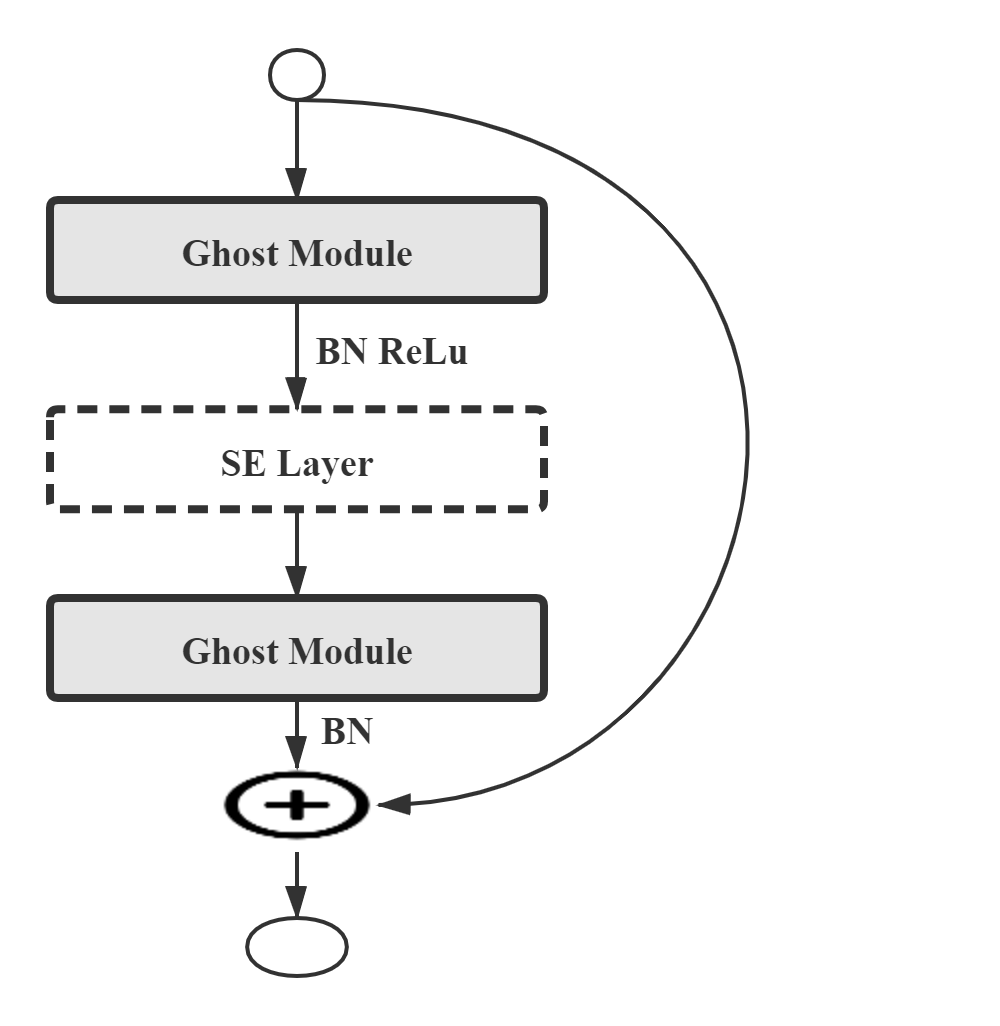
\includegraphics[width=\textwidth]{thesis-template-master/images/stride1 module.png}
			\caption{Stride = 1 SE = 0 G-bneck}
			\label{fig:cellnet}
		\end{subfigure}
		\begin{subfigure}[b]{0.49\textwidth}
		    \centering
			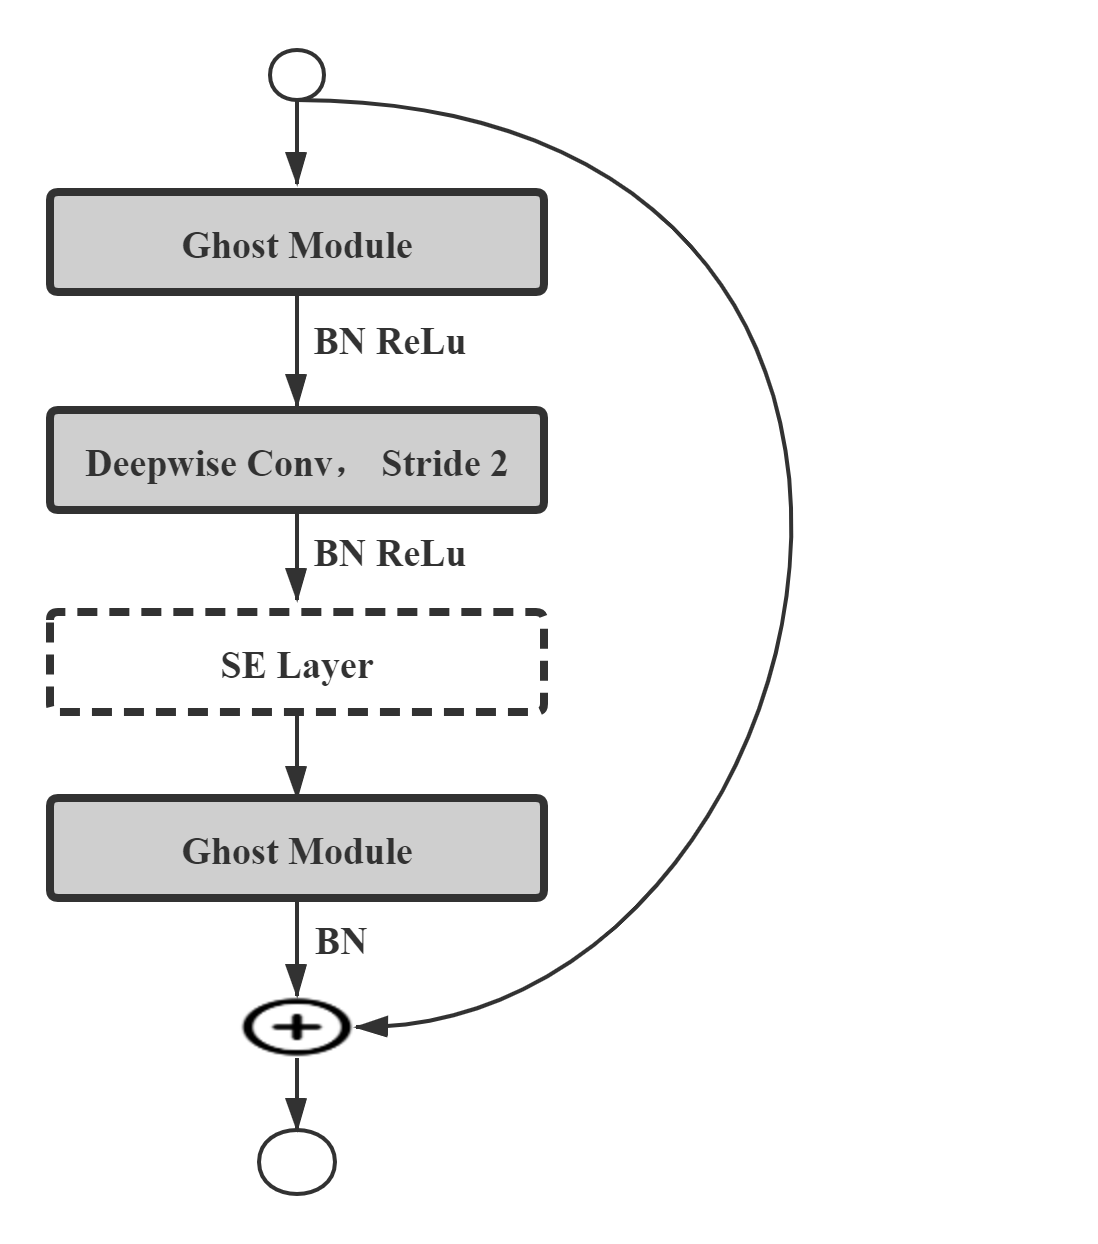
\includegraphics[width=\textwidth]{thesis-template-master/images/stride2 module.png}
			\caption{Stride = 2 SE = 0 G-bneck}
			\label{fig:cellnet}
		\end{subfigure}
	\end{center}
	\caption{\textbf{Two kind of Gbnecks we proposed for feature extraction}.We apply Stride = 1 to keep the output channel of the feature map, Stride = 2 decreases the output channel while extracting information without losing a lot of information. SE = 0 represents not applying SE layer.  The short cut is used to connect between the inputs and outputs of these two Ghost modules, as suggested by GhostNet, we implement in th short-cut of Stride=2 G-bneck by a down sampling layer, not only single connection in short-cut of Stride =1 G-bneck.}
\end{figure}

\begin{figure}[h]
	\begin{center}
		\begin{subfigure}[b]{\textwidth}
		    \centering
			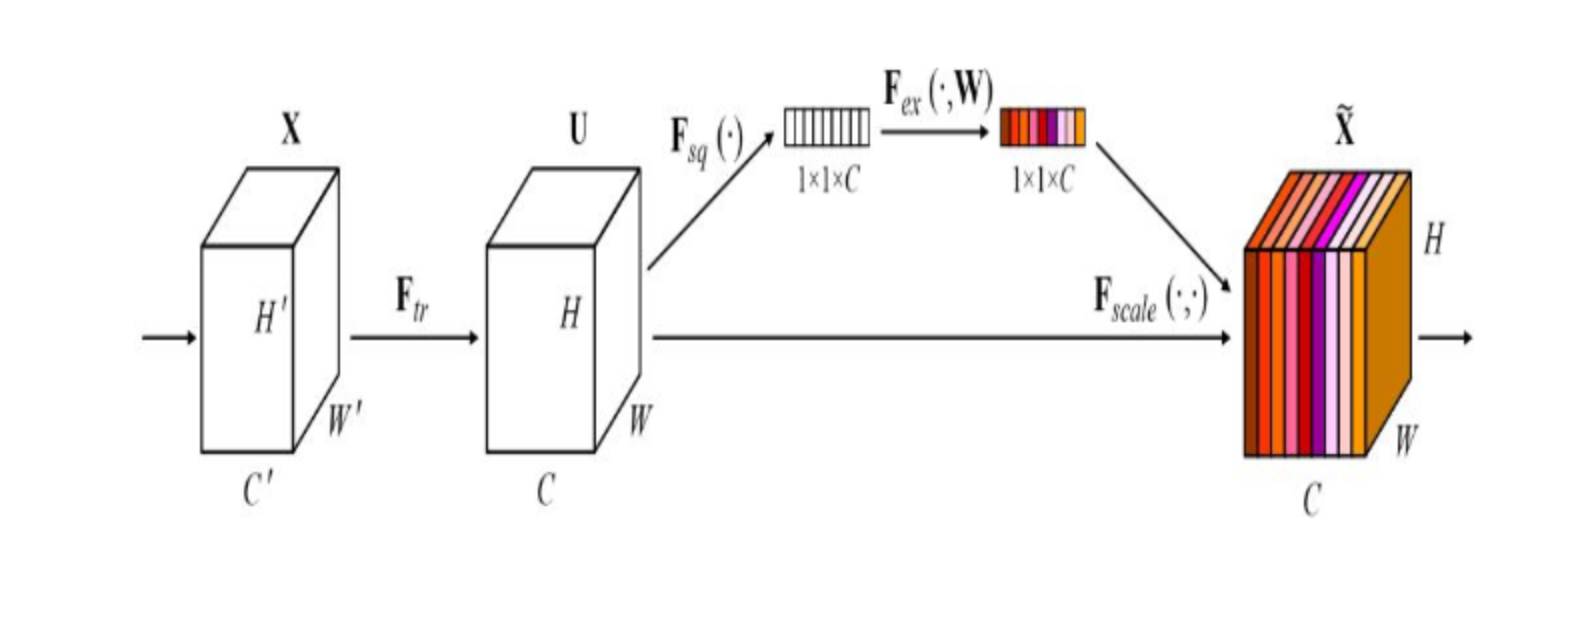
\includegraphics[width=\textwidth]{thesis-template-master/images/SElayer.png}
			\label{fig:cellnet}
		\end{subfigure}
	\end{center}
	\caption{\textbf{SE Layer}.}
\end{figure}

\subsection{Squeeze-and-Excitation (SE Layer)} % (fold)
\label{sub:amet}

\textbf{scaling inhibiting vs intrinsic features map.} Squeeze-and-Excitation (SE)\cite{b24} adaptively recalibrates channel-wise feature responses by explicitly modeling inter-dependencies between channels. 

SENet further demonstrated that SE blocks bring significant improvements in performance for existing state-of-the-art CNNs with slight additional computational cost \cite{b24}. 



\subsection{Analysis on complexities and necessities} % (fold)
\label{sub:dolor_sit}
Here, we further analyze the profit on memory usage and theoretical speed-up by employing the Ghost module, in additional we will plot the visual experiments. The theoretical speed-up ratio $\gamma$ of upgrading ordinary convolution with the Ghost module is equal to following:

\begin{equation}
\begin{split}
\gamma $& = \frac{\left ( n\cdot {h}'\cdot {w}'\cdot c\cdot k\cdot k \right )}{\left (\frac{n}{s}\cdot {h}'\cdot {w}'\cdot c\cdot k\cdot k +\left ( s-1 \right )\cdot \frac{n}{s}\cdot {h}'\cdot {w}' \cdot d\cdot d \right )} \\
$&= \frac{c\cdot k\cdot k}{\frac{1}{s}\cdot c\cdot k\cdot k + \frac{s-1}{s}\cdot d\cdot d } \\
$&\approx \frac{s\cdot c}{s +c-1 } \\
$&\approx s $\label{speed}
\end{split}
\end{equation}

In Equation \eqref{speed}, ${h}' \cdot {w}' \cdot {n}$ represents  $n$ output feature maps with height ${h}'$, width ${w}'$, and $k \cdot k$, $d \cdot d$ stands for the convolution kernel filter and linear operation kernel size, respectively. And $m$ is the number of intrinsic feature maps, where $m < n$ because we only take few intrinsic feature maps and apply a series of cheap linear operations on each intrinsic feature to generate $s$ ghost features. It is also noteworthy that there are 1 ghost map adopted by identify mapping that indicates $s-1$. In total there are $\frac{n}{s} \cdot(s-1)$  linear operations. This leads to theoretically $s$ speed-up ratio.

More feature maps generated by linear operation based on a set of intrinsic feature maps, instead of generating a lot of redundant data by point-wise convolution which takes huge amount of parameters simultaneously. This also partially explains that our net achieves the best performance on several benchmarks shown in Table 2 and Table 3.
As far as we deeply analyze each-layer-generated feature map by our net, we can also figure out the second factor: the artifacts appear in the image could also be learned by the neural network, which greatly affects the accuracy of the network, with the combination of AttentionNet segmentation techniques in cell image pre-processing, we can more focus on object rather than artifacts.


\begin{table}[htbp]
\centering

\scalebox{0.9}{
\begin{tabular}{@{}llllllll@{}}
\toprule
layer & Type    & Filters & Size/Stride           & Input      & Output     & \multicolumn{1}{l}{\#Expan} & SE \\ \midrule
0     & Conv2d  & 64      & 3\times3/2                 & 416\times416\times3  & 112\times112\times64 & -                                  & -  \\
1     & Maxpool & -       & 3\times3/2                 & 112\times112\times64 & 56\times56\times64   & -                                  & -  \\
2     & G-bneck & 64      & 3\times3/1                 & 56\times56\times64   & 56\times56\times64   & 64                                 & 0  \\
3     & G-bneck & 64      & 3\times3/1                 & 56\times56\times64   & 56\times56\times64   & 64                                 & 0  \\
4     & G-bneck & 64      & 3\times3/1                 & 56\times56\times64   & 56\times56\times64   & 128                                & 1  \\
5     & G-bneck & 128     & 3\times3/2                 & 56\times56\times64   & 28\times28\times128  & 256                                & 0  \\
6     & G-bneck & 128     & 3\times3/1                 & 28\times28\times128  & 28\times28\times128  & 512                                & 1  \\
7     & G-bneck & 256     & 3\times3/2                 & 28\times28\times128  & 14\times14\times256  & 1024                               & 0  \\
8     & G-bneck & 256     & 3\times3/1                 & 14\times14\times256  & 14\times14\times256  & 1024                               & 1  \\
9     & G-bneck & 512     & 3\times3/2                 & 14\times14\times256  & 7\times7\times512    & 1024                               & 0  \\
10    & Conv2d  & 512     & 1\times1/1                 & 7\times7\times512    & 7\times7\times512    & -                                  & -  \\
11    & Advpool & -       & 7\times7                   & 7\times7\times512    & 1\times1\times512    & -                                  & -  \\
12    & Conv2d  & 512     & 1\times1/1                 & 1\times1\times512    & 1\times1\times512    & -                                  & -  \\
13    & FC      & -       & \multicolumn{1}{c}{-} & 1\times1\times512    & 1000       & -                                  & -  \\ \bottomrule


\end{tabular}}
\caption{\textbf{CellNet Network Structure}. G-bneck denotes novel Ghostbottleneck. \#Expan means expansion size.}
\end{table}
































\chapter{Experiments}
\label{sec:examples}
In this chapter, we put the focus on experimentally evaluating our proposed two architectures. At the very beginning, we will introduce the standard evaluation metrics,such as Confusion Matrix, F1 Score, Area Under the ROC curve(AUC – ROC), Top-1 accuracy, mAP,  weights and FLOPs and so on. 

Followed by qualitative and quantitative results on two well-established benchmark data sets(Cifar-10 for standard classification task, Pneumonia dataset for biomedical classification task), we also contribute to the work of the establishing the first ever Sezary Sydrome dataset benchmark, including the data acquisition, handling, aggregating and pre-processing with our AttentionNet to classifier data into the unique and corresponding folder. Among the well-established benchmark, we additionally made the COVID-19 Xray/CT image dataset while participating the kaggle challenge fighting against the COVID-19. We then report new state-of-the-art results on all these four data sets. We also  provide detailed descriptions on the training and testing pipeline, including data preprocessing, training tricks and strategies as well as network architectures used to obtain the final scores.

\section{Evaluation Metrics}
\label{sec:lorem}
In order to quantitatively evaluate the performance of a model, we define Evaluation metrics suit for our cases.

To start with  our AttentionNet,  as described in the section3 , the AttentionNet  is  based on classification task and follows the superiority of the architecture of Yolov3- tiny, therefore, there is  generally established metric for evaluation, such as Confusion Matrix Precision and Recall, F1 Score, mAP,  the IOU and  Classification Loss. In order  to compare our methods on new dataset we established, we therefore adopted most of those evaluation schemes from the original YOLOv3. In addition, combining Area Under the ROC curve leads to conclusive quality metrics paying attention to various aspects. 
In further, we consider the resources limitation and time cost for software application in real scenarios usages, we then analyzed  the time cost in different GPU avail-abilities and computation FLOPs.


\subsection{Confusion Matrix}
In order to make quantitative statements about the model of  the CellNet, we mainly utilized the  Confusion Matrix (TP, TN, FP, FN, Sensitivity, Accuracy) , time complexity, weights of parameters and the computation complexity FLOPs. 
Evaluation metrics are the means to perform this comparison which is presented in the following paragraphs. The notation is adopted from Zhao et al.

A confusion matrix is an $N \times N$ matrix, where $N$ is the number of classes being predicted. because we have binary classification problem, we set then the $N=2$, and hence we get a $2 \times 2$ matrix. Here are a few definitions:


\begin{table}[h]
\centering
\scalebox{0.8}{
\begin{tabular}{|l|l|l|l|l|}
\hline
\multicolumn{2}{|c|}{\multirow{2}{*}{\textbf{}}}                                                & \multicolumn{2}{c|}{\textbf{Target}}                                                                                                  & \multirow{2}{*}{}    \\ \cline{3-4}
\multicolumn{2}{|c|}{}                                                                          & Positive                                                          & Negative                                                          &                      \\ \hline
\multirow{2}{*}{\textbf{\begin{tabular}[c]{@{}c@{}}Model\\ Prediction\end{tabular}}} & Positive & TP                                                                & FP                                                                & Precision (TP/(TP+FP)) \\ \cline{2-5} 
                                                                                     & Negative & FN                                                                & TN                                                                & Recall (TN/(FN+TN))   \\ \hline
\multicolumn{2}{|l|}{}                                                                          & \begin{tabular}[c]{@{}l@{}}Sensitivity \\ (TP/(TP+FN))\end{tabular} & \begin{tabular}[c]{@{}l@{}}Specificity \\ (TN/(FP+FN))\end{tabular} &                      \\ \hline

\end{tabular}}

\caption{\textbf{The illustration of  Confusion Matrix}. We will use the precision and recall as evaluation matrix in our experiments.}

\end{table}

The number of true positives ($TP$) constitutes how many data points of the ground
truth class $c$ were correctly classified:


\begin{equation}
\begin{split}
TP\left ( Y_{p},Y_{g},c \right )=\sum_{x}^{}Y_{p}\left ( x,c \right )\times Y_{g}\left ( x, c \right )
\label{}
\end{split}
\end{equation}
where the ground truth class distribution $Y_{g} (x, c)$
and the predicted class distribution $Y_{p} (x, c)$ which both yield $1$ if the data point $x$  is classified as class $c$.

\begin{equation}
\begin{split}
TN\left ( Y_{p},Y_{g},c \right )=\sum_{x}^{}\left (1-Y_{p}\left ( x,c \right )  \right )\times \left ( 1-Y_{g}\left ( x,c \right ) \right ) 
\label{}
\end{split}
\end{equation}

The number of true negatives ($TN$) comprises how many data points not belonging to
the ground truth class $c$ were correctly rejected by the predictor.

\begin{equation}
\begin{split}
FP\left ( Y_{p},Y_{g},c \right )=\sum_{x}^{}Y_{p}\left ( x,c \right )\times \left ( 1-Y_{g}\left ( x,c \right ) \right )
\label{}
\end{split}
\end{equation}

The number of false positives ($FP$) represents how many data points not belonging to the ground truth class c were wrongly classified by the predictor.
The final metric is the number of false negatives ($FN$) which represents how many data points of the ground truth class c were wrongly rejected by the predictor:
\begin{equation}
\begin{split}
FN\left ( Y_{p},Y_{g},c \right )=\sum_{x}^{}\left (1-Y_{p}\left ( x,c \right )  \right )\times Y_{g}\left ( x,c \right ) 
\label{}
\end{split}
\end{equation}


Another metric we are interested in is precision, which measures the ratio between true positives and the overall number of class instantiations. Precision returns a probability estimate of how exact our predictor is and it returns the proportion of positive cases that were correctly identified. Besides precision, there is the metric of recall which is defined as the fraction of true positives to the overall positive samples. This estimates how complete a prediction is, as it generates  the proportion of negative cases that were correctly identified.

In general we are concerned with more than one of the above defined metric.
A high precision rate therefore states that positive predictions are likely to be classified correctly. Contrastingly, the recall rate measures how complete a prediction is. Hence, a high recall rate means that instantiations of a specific class are likely to be detected in the dataset.

However, we favor a scalar value to create an ordered ranking of algorithms performing on the same task. We thus condense both metrics into a single one. The $F$ score  measure weights precision and recall according to a weighting factor such that recall has $\beta$ times more weight than precision:
\begin{equation}
\begin{split}
F_{\beta }=\left ( 1+\beta ^{2} \right )\times \frac{precision\times recall}{\left (\beta ^{2}\times precision \right )+recall }
\label{}
\end{split}
\end{equation}

In the case of $ \beta = 1$ , the $F_{1 }$ score is the harmonic mean between precision and recall.

Positively correlated to F score is the metric of intersection over union (IoU) which is prominent in the field of computer vision and is used in the evaluation protocols across all tested datasets of this thesis.




\subsection{ROC curve and AUC (Area under Curve)}
The ROC (Receiver operating characteristic) curve is the plot between sensitivity and (1- specificity). As shown in Table 4.1, the sensitivity of a test is also called the true positive rate (TPR) and stands for the proportion of actual positive cases which are correctly identified. For example, a test that correctly identifies all positive samples in a panel is very sensitive. Another test that only detects 60 \% of the positive samples in the panel would be deemed to have lower sensitivity as it is missing positives and giving higher a false negative rate (FNR).

The specificity of a test, also referred to as the true negative rate (TNR), is the proportion of samples that test negative and are genuinely negative. For example, a test that identifies all healthy people as being negative for a particular illness is very specific. Another test that incorrectly identifies 30 \% of healthy people as having the condition would be deemed to be less specific, having a higher false positive rate (FPR).

(1- specificity) is also known as false positive rate (FNR). ROC curve on the other hand is almost independent of the response rate. This is because it has the two axis coming out from columnar calculations of confusion matrix.

\begin{figure}[h]
	\begin{center}
		\begin{subfigure}[b]{\textwidth}
		    \centering
			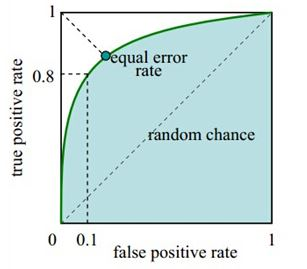
\includegraphics[width=0.4\textwidth]{thesis-template-master/images/ROC.JPG}
			\label{fig:cellnet}
		\end{subfigure}
	\end{center}
	\caption{\textbf{ROC (Receiver operating characteristic) curve}.$x$ axis in ROC curve represents FPR, or 1-TNR, or 1-Specificity. The greater the FPR, the more actual negative categories in the predicted positive category. On the other hand, $y$ axis in ROC curve represents TPR or by another word Sensitivity. The greater the TPR, the more actual positive categories in the predicted positive category.}
\end{figure}
Our idea objective will be TPR=1 and FPR=0, which is the (0,1) point in the figure, so the closer the ROC curve is to the (0,1) point, the better it deviates from the diagonal of 45 degrees, and the greater the Sensitivity and Specificity, the more effective.
The numerator and denominator of both x and y axis will change on similar scale in case of response rate shift.

The biggest advantage of using ROC curve is that it is independent of the change in proportion of responders. This statement will get clearer in the following sections.

As a numerical value, AUC(Area under Curve) can directly evaluate the quality of the classifier and it calculates the area under the ROC curve varies from 0 and 1. A test with no better accuracy than chance has an AUC of 0.5, a test with perfect accuracy has an AUC of 1.

The interpretation of the AUC is the average value of sensitivity for all possible values of specificity. for make it clear, we illustrated with a binary  classification problem. By randomly given a positive sample and a negative sample. AUC represents the probability of the classifier predicting positive samples is greater than the probability of the classifier predicting negative samples.%AUC评估的是随机给定一个正样本和一个负样本,模型对正样本的预测概率大于模型对于负样本预测概率的概率


\subsection{Top N accuracy }
Top N accuracy is not any different metric, but it’s just standard accuracy of the true class being equal to any of the N most probable classes predicted by the classification model.
Top 1 accuracy is the accuracy where true class matches with the most probable classes predicted by the model, which is the same as our standard accuracy. Top 2 accuracy is the accuracy where true class matches with any one of the 2 most probable classes predicted by the model. And accordingly, the Top 3 accuracy is the accuracy where true class matches with any one of the 3 most probable classes predicted by the model. In the same way, we can measure the top 4, top 5, top 6, and so on.


We illustrate both metrics in the following examples considering  classifying records into respective animals (dog, cat, lion, tiger, and elephant). The following table shows the true target class and predicted class of 6 records.
For instance, if the test target class is given Dog, the true class under the Top 1 accuracy circumstance is unmatched with the most probable classes predicted by the model{Cat}. Therefore, this can be recognized as false prediction and that leads to 50\% Top 1 accuracy.
on the other hand, the true class under the Top 2 accuracy circumstance is unmatched with the most 2 probable classes predicted by the model{Cat, Dog}.because only one matched, we can count them as positive prediction, it leads to 83\% on Top  1  accuracy.
\begin{table}[h]
\centering

\begin{tabular}{@{}cccc@{}}

\toprule
\multicolumn{2}{c}{Top-1 accuracy: 0.5} & \multicolumn{2}{c}{Top-2 accuracy: 0.83} \\ \midrule
Test Target class    & Prediction      & Test Target class   & Prediction         \\
Dog                  & \{Cat\}         & Dog                 & \{Cat, Dog\}       \\
Elephant             & \{Elephant\}    & Elephant            & \{Elephant, Cat\}  \\
Lion                 & \{Tiger\}       & Lion                & \{Tiger, Cat\}     \\
Dog                  & \{Dog\}         & Dog                 & \{Dog, Lion\}      \\
Lion                 & \{Lion\}        & Lion                & \{Lion, Cat\}      \\
Tiger                & \{Cat\}         & Tiger               & \{Cat, Tiger\}     \\ \bottomrule


\end{tabular}

\caption{\textbf{The illustration of Top 1 accuracy and Top 2 accuracy}. As Table illustrated, we will obtain an accuracy of 50\% on Top 1 accuracy and 83\% on Top 1 accuracy. }
\end{table}


As Table illustrated, we will obtain an accuracy of 50\%, when  we taking the Top 1 accuracy into evaluation metrics, which is not so satisfying. As soon as we take into consideration of the accuracy where where true class matches with any one of the 2 most probable classes predicted by the model, as the second column demonstrated, we will be getting an accuracy of 83\%, which is a significant increase compared to the previous one. this is the basic intuition behind finding the Top N accuracy. which is especially  applicable for the mutil-class objects prediction tasks.





\section{Sezary Sydrome Dataset}
\label{sec:lorem}

\begin{figure}[h]
	\begin{center}
		\begin{subfigure}[b]{\textwidth}
		    \centering
			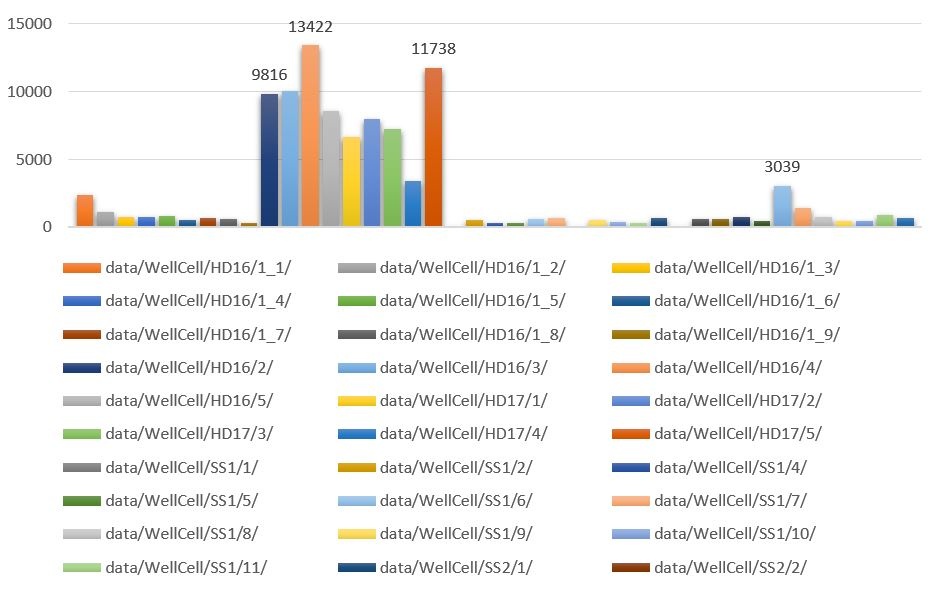
\includegraphics[width=0.9\textwidth]{thesis-template-master/images/wellcellSezary dataset.JPG}
			\label{fig:cellnet}
		\end{subfigure}
	\end{center}
	\caption{\textbf{Wellcell dataset on Sezary dataset}. In total we had Well cell data:$HD16:49787+ HD17:37009+SS1:5250+SS2:10852= 102,898$.}
\end{figure}

\begin{figure}[h]
	\begin{center}
		\begin{subfigure}[b]{\textwidth}
		    \centering
			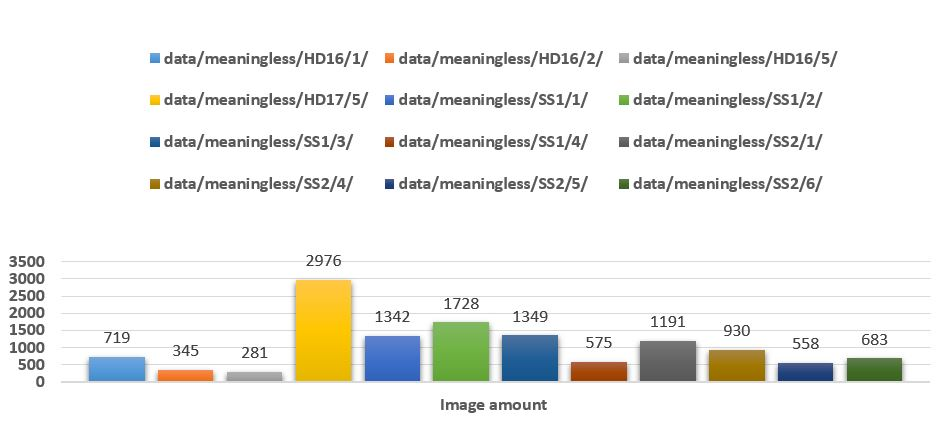
\includegraphics[width=0.9\textwidth]{thesis-template-master/images/noiseofSezarySyndrome.JPG}
			\label{fig:cellnet}
		\end{subfigure}
	\end{center}
	\caption{\textbf{Noise dataset of SezarySyndrome}.We had noise data: 12,695.}
\end{figure}

\subsection{The introduction of Sezary Sydrome Dataset}
Sezary syndrome is an aggressive form of cutaneous T-cell lymphoma which is a group of disorders that occur when T-cells (a type of white blood cell) become cancerous and affect the skin\cite{Alain}. Moreover, it corresponds to 3\% of all cutaneous lymphomas, and it is characterized by a triad of manifestations: erythrodermia with pruritus, limphonodomegalia and atypical circulating lymphocytes (referred to as Sézary or Lutzner cells). Associated clinical manifestations include lagophthalmos, alopecia, palmoplantar hyperkeratosis and onycodystrophy.\cite{Yamashita}


\begin{figure}[ht]
	\begin{center}
		\begin{subfigure}[b]{0.25\textwidth}
			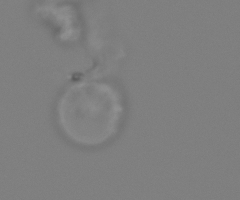
\includegraphics[width=\textwidth]{thesis-template-master/images/noisefortest (106).png}
			\label{fig:Debris}
		\end{subfigure}
		\begin{subfigure}[b]{0.25\textwidth}
			\reflectbox{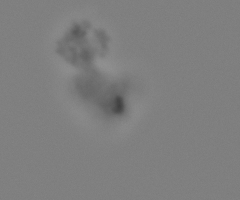
\includegraphics[width=\textwidth]{thesis-template-master/images/noisefortest (107).png}}
			\label{fig:Out of Focus}
		\end{subfigure}
		\begin{subfigure}[b]{0.25\textwidth}
			\reflectbox{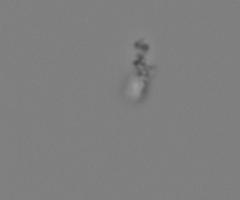
\includegraphics[width=\textwidth]{thesis-template-master/images/noisefortest (47).png}}
			\label{fig:Lighting Artifacts}
		\end{subfigure}
		\begin{subfigure}[b]{0.25\textwidth}
			\reflectbox{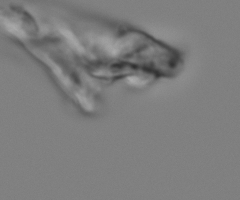
\includegraphics[width=\textwidth]{thesis-template-master/images/noisefortest (66).png}}
			\label{fig:Outside FOV}
		\end{subfigure}
		\begin{subfigure}[b]{0.25\textwidth}
			\reflectbox{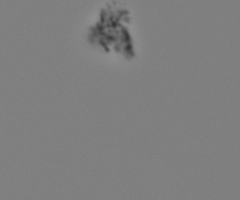
\includegraphics[width=\textwidth]{thesis-template-master/images/noisefortest (69).png}}
			\label{fig:Contaminated}
		\end{subfigure}
		\begin{subfigure}[b]{0.25\textwidth}
			\reflectbox{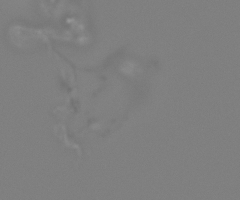
\includegraphics[width=\textwidth]{thesis-template-master/images/noisefortest (91).png}}
			\label{fig:Good Cell}
		\end{subfigure}
		\begin{subfigure}[b]{0.25\textwidth}
			\reflectbox{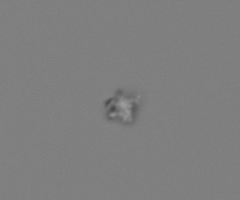
\includegraphics[width=\textwidth]{thesis-template-master/images/noisefortest (93).png}}
			\label{fig:Good Cell}
		\end{subfigure}
		\begin{subfigure}[b]{0.25\textwidth}
			\reflectbox{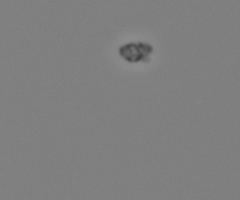
\includegraphics[width=\textwidth]{thesis-template-master/images/noisefortest (87).png}}
			\label{fig:Good Cell}
		\end{subfigure}
				\begin{subfigure}[b]{0.25\textwidth}
			\reflectbox{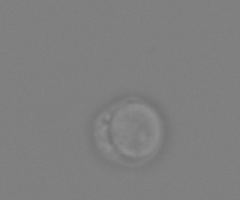
\includegraphics[width=\textwidth]{thesis-template-master/images/ss5 (1).png}}
			\label{fig:Good Cell}
		\end{subfigure}
	\end{center}
	\caption{Meaningless noise images from Sezary Syndrome data set.  The six typical  noise images introduced in Figure 1.1. In total we had noise data: 12,695.}
	\label{fig:lennas}
\end{figure}

Sezary syndrome symptoms is characterized by a widespread red rash that may cover most of the body, the presence of cancerous T cells (called Sezary cells) in the blood, and abnormally enlarged lymph nodes. Other signs and symptoms may include intense itchiness, scaling and peeling of the skin; fever; weight loss; hair loss; outward turning of the eyelids (ectropion). According to \cite{10.1182/blood-2004-09-3502}\cite{20001195667}, the behaviour of the Sezary syndrome is aggressive with a median survival of 1–5 years  and the exact cause of Sezary syndrome is currently unknown. Treatment varies based on the signs and symptoms present in each person and the severity of the condition.\cite{Yamashita}

A diagnosis of Sezary syndrome is often suspected in people with characteristic signs and symptoms. Additional testing can then be ordered to confirm the diagnosis. This may include: A skin biopsy, A complete blood count, Peripheral blood smear, Immunophenotyping, T-cell receptor (TCR) gene rearrangement test and Flow cytometry \cite{Alain}.


\begin{figure}[ht]
	\begin{center}
		\begin{subfigure}[b]{0.25\textwidth}
			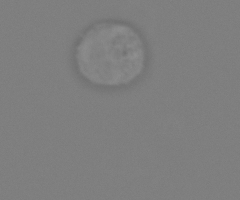
\includegraphics[width=\textwidth]{thesis-template-master/images/hd7 (80).png}
			\label{fig:Debris}
			\caption{HD cell}
		\end{subfigure}
		\begin{subfigure}[b]{0.25\textwidth}
			\reflectbox{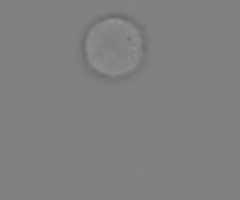
\includegraphics[width=\textwidth]{thesis-template-master/images/hd7 (107).png}}
			\label{fig:Out of Focus}
			\caption{HD cell}
		\end{subfigure}
		\begin{subfigure}[b]{0.25\textwidth}
			\reflectbox{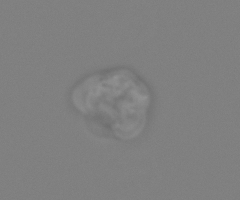
\includegraphics[width=\textwidth]{thesis-template-master/images/hd7 (102).png}}
			\label{fig:Lighting Artifacts}
			\caption{HD cell}
		\end{subfigure}
		\begin{subfigure}[b]{0.25\textwidth}
			\reflectbox{\includegraphics[width=\textwidth]{thesis-template-master/images/ss5 (135).png}}
			\label{fig:Outside FOV}
			\caption{SS cell}
		\end{subfigure}
		\begin{subfigure}[b]{0.25\textwidth}
			\reflectbox{\includegraphics[width=\textwidth]{thesis-template-master/images/ss5 (120).png}}
			\label{fig:Contaminated}
			\caption{SS cell}
		\end{subfigure}
		\begin{subfigure}[b]{0.25\textwidth}
			\reflectbox{\includegraphics[width=\textwidth]{thesis-template-master/images/ss5 (24)}}
			\label{fig:Good Cell}
			\caption{SS cell}
		\end{subfigure}
		
	\end{center}
	\caption{Well cell images from Sezary Syndrome data set. Only Well cell images from Sezary Syndrome data set can be analyzed in classification task. As shown in the figure, the morphological characteristics can be even hardly distinguish by experts, which partly explains the unsatisfied classification accuracy of neural network. In total we had well cell data: 102,898.}
	\label{fig:lennas}
\end{figure}

Based on previously manually bag-labeled image, we manipulated the second round of filtering, because of the impurity of the data set. This is actually final data set amount. Because we do not allow the cell folder contains obviously noise data, so we manually checked for the whole data set again and deleted those impure images, the following data is the newest version of the folder(Seen figure 4.2 and figure 4.3). 



\subsection{AttentionNet on Sezary Sydrome Dataset}

\begin{table}[b]
\scalebox{0.5}{
\begin{tabular}{@{}ccl@{}}
\toprule
Configuration hyperparameter         & Value                                                                                                & Annotation                                                                                                                                                                                                                                                                                                                                                                                             \\ \midrule
\multicolumn{1}{|c|}{batch}          & \multicolumn{1}{c|}{64}                                                                              & \multicolumn{1}{l|}{Update parameters every batch of 64 samples}                                                                                                                                                                                                                                                                                                                                       \\ \midrule
\multicolumn{1}{|c|}{subdivisions}   & \multicolumn{1}{c|}{1}                                                                               & \multicolumn{1}{l|}{\begin{tabular}[c]{@{}l@{}}The batch will be divided by 1 to decrease GPU VRAM requirements \\ as we are using ETH Leonhard we donot facing the GPU resources limitations\end{tabular}}                                                                                                                                                                                            \\ \midrule
\multicolumn{1}{|c|}{height}         & \multicolumn{1}{c|}{416}                                                                             & \multicolumn{1}{l|}{The width of input figure}                                                                                                                                                                                                                                                                                                                                                         \\ \midrule
\multicolumn{1}{|c|}{width}          & \multicolumn{1}{c|}{416}                                                                             & \multicolumn{1}{l|}{The height of input figure}                                                                                                                                                                                                                                                                                                                                                        \\ \midrule
\multicolumn{1}{|c|}{channels}       & \multicolumn{1}{c|}{3}                                                                               & \multicolumn{1}{l|}{\begin{tabular}[c]{@{}l@{}}The channels of input training images,\\ as our image is here RGB image, therefore, we set here 3\end{tabular}}                                                                                                                                                                                                                                         \\ \midrule
\multicolumn{1}{|c|}{momentum}       & \multicolumn{1}{c|}{0.9}                                                                             & \multicolumn{1}{l|}{\begin{tabular}[c]{@{}l@{}}For the poorly conditioned Hessian matrix problem \\ (intuitively, the gradient is highly sensitive to certain directions of the parameter space)\\ usually set 0.5, 0.9, or 0.99, which means the maximum speed is \\ 2 times, 10 times, 100 times the algorithm of SGD\end{tabular}}                                                                  \\ \midrule
\multicolumn{1}{|c|}{decay}          & \multicolumn{1}{c|}{0.0005}                                                                          & \multicolumn{1}{l|}{Regularization term of weight decay  to prevent overfitting}                                                                                                                                                                                                                                                                                                                       \\ \midrule
\multicolumn{1}{|c|}{angle}          & \multicolumn{1}{c|}{0}                                                                               & \multicolumn{1}{l|}{Generate more training samples by rotation}                                                                                                                                                                                                                                                                                                                                        \\ \midrule
\multicolumn{1}{|c|}{saturation}     & \multicolumn{1}{c|}{1.5}                                                                             & \multicolumn{1}{l|}{Generate more training samples by adjusting saturation}                                                                                                                                                                                                                                                                                                                            \\ \midrule
\multicolumn{1}{|c|}{exposure}       & \multicolumn{1}{c|}{1.5}                                                                             & \multicolumn{1}{l|}{Generate more training samples by adjusting exposure}                                                                                                                                                                                                                                                                                                                              \\ \midrule
\multicolumn{1}{|c|}{hue}            & \multicolumn{1}{c|}{.1}                                                                              & \multicolumn{1}{l|}{Generate more training samples by adjusting hue}                                                                                                                                                                                                                                                                                                                                   \\ \midrule
\multicolumn{1}{|c|}{learning rate}  & \multicolumn{1}{c|}{0.001}                                                                           & \multicolumn{1}{l|}{\begin{tabular}[c]{@{}l@{}}Initial learning rate, The learning rate determines how fast the parameter moves to the optimal solution. \\ If it is too large, it may cross the optimal value and cause the model to fail to converge. \\ Otherwise if it is too small, the algorithm cannot converge for a long time \\ and it is easy to fall into the local optimal.\end{tabular}} \\ \midrule
\multicolumn{1}{|c|}{max batches}    & \multicolumn{1}{c|}{500200}                                                                          & \multicolumn{1}{l|}{Stop learning after training reaches max\_batches}                                                                                                                                                                                                                                                                                                                                 \\ \midrule
\multicolumn{1}{|c|}{policy}         & \multicolumn{1}{c|}{steps}                                                                           & \multicolumn{1}{l|}{\begin{tabular}[c]{@{}l@{}}The policies for adjusting the learning rate are as follows:\\ CONSTANT, STEP, EXP, POLY, STEPS, SIG, RANDOM\end{tabular}}                                                                                                                                                                                                                              \\ \midrule
\multicolumn{1}{|c|}{steps}          & \multicolumn{1}{c|}{400000,450000}                                                                   & \multicolumn{1}{l|}{Adjust the learning rate according to batch\_num}                                                                                                                                                                                                                                                                                                                                  \\ \midrule
\multicolumn{1}{|c|}{scales}         & \multicolumn{1}{c|}{.1,.1}                                                                           & \multicolumn{1}{l|}{The rate of change in learning rate, cumulatively multiplied}                                                                                                                                                                                                                                                                                                                      \\ \midrule
\multicolumn{1}{|c|}{mask}           & \multicolumn{1}{c|}{1,2,3,4,5,67,8,9}                                                                & \multicolumn{1}{l|}{Yolo Output Layer will select different three anchor box set}                                                                                                                                                                                                                                                                                                                      \\ \midrule
\multicolumn{1}{|c|}{anchors}        & \multicolumn{1}{c|}{\begin{tabular}[c]{@{}c@{}}38,39 50,53\\ 51,67 71,78\\ 84,83 99,95\end{tabular}} & \multicolumn{1}{l|}{\begin{tabular}[c]{@{}l@{}}The prior prediction box learned from our KMeans++cluster \\ one set contains two value (w,h)\end{tabular}}                                                                                                                                                                                                                                             \\ \midrule
\multicolumn{1}{|c|}{classes}        & \multicolumn{1}{c|}{2}                                                                               & \multicolumn{1}{l|}{The number of object classes that the network needs to classifier}                                                                                                                                                                                                                                                                                                                 \\ \midrule
\multicolumn{1}{|c|}{num}            & \multicolumn{1}{c|}{6}                                                                               & \multicolumn{1}{l|}{Each grid cell predicts \#num number of bounding boxes}                                                                                                                                                                                                                                                                                                                            \\ \midrule
\multicolumn{1}{|c|}{jitter}         & \multicolumn{1}{c|}{0.3}                                                                             & \multicolumn{1}{l|}{Increase noise by jitter to suppress overfitting}                                                                                                                                                                                                                                                                                                                                  \\ \midrule
\multicolumn{1}{|c|}{ignore\_thresh} & \multicolumn{1}{c|}{0.7}                                                                             & \multicolumn{1}{l|}{The parameter determines whether the IOU error needs to be calculated  in the cost function}                                                                                                                                                                                                                                                                                       \\ \midrule
\multicolumn{1}{|c|}{truth\_thresh}  & \multicolumn{1}{c|}{1}                                                                               & \multicolumn{1}{l|}{The size of the IOU threshold involved in the calculation}                                                                                                                                                                                                                                                                                                                         \\ \midrule
\multicolumn{1}{|c|}{random}         & \multicolumn{1}{c|}{1}                                                                               & \multicolumn{1}{l|}{Multi-scale training is enabled. Otherwise, the training size of image is the same as the input size}                                                                                                                                                                                                                                                                              \\ \bottomrule
\end{tabular}}
\caption{ \textbf{AttentionNet configuration files (.cfg) }. As shown in the evaluation table, we will present here the training hyper-parameters that we chooses indetails and explained the reason why we set like that.}
\end{table}


\subsubsection{Implementation and Hyper-parameters}

\textbf{Preparing dataset.} Before starting to train, we prepare the data for object detection. we used LabelImg tool to formulate the expert defined good cell/noise shapes. In this tool we can prepare our data in two different format: xml and txt. For the suggestion of original yolov3, we used txt format. We also wrote a function (xmltotxt.py) can basically convert the xml format to txt format. 

Any machine learning training procedure involves first splitting the data randomly into two sets. By using our (filtertrainandtest.py) script we can split the test and train data set into user defined distribution. Training set: this is the part of the data on which we train the model. Test set : This is the part of the data on which we test our model. Typically, this is 10-30\% of the data. No image should be part of the both the training and the test set.

Then we create two file named train.txt and test.txt. These files must contain path of train and test images in data set line by line. Train.txt should have the formal: $(data/images/imagenames.png)$ and Test.txt should have the formal $(data/images/imagenames.png)$.

Because we are supervised learning, we should also generate (./image) and (. /labels) folder accordingly. Moreover, the label file and the image should have same filename. This can be guarantee by our script (xmltotxt.py).

\textbf{Preparing AttentionNet configuration files}. YOLOv3 needs certain specific files to know how and what to train. We must create these three files(.data, .names, and .cfg) and we explain those configuration hyper parameters in the above table 4.3\\

\subsubsection{Evaluated performances}
With help of Cycle detection and more Cell data be manually labeled, We trained 1000 epochs We input 857 instance level-labeled image,which we set up 772(90\%) image for train set, and 85 images for test. For Training image: 772 images consists of 274 noise image , 144 HD Cell image and  439 SS cell image. Val image: 85 image, In addition, we test the trained model on 723 new image as well.


\begin{figure}[h]
	\begin{center}
		\begin{subfigure}[b]{\textwidth}
		    \centering
			\includegraphics[width=1\textwidth]{thesis-template-master/images/cellyolo best weight based on manually labeled 1500 images.png}
			\label{fig:cellnet}
		\end{subfigure}
	\end{center}
	\caption{\textbf{The demonstration of train performance of CellYolo best weight based on manually labeled 1500 images}. The P value is nearly 85\% and the F1 value is also quite well, the mAP@0.5 achieves nearly 88\%.}
\end{figure}

\begin{figure}[h]
	\begin{center}
		\begin{subfigure}[b]{\textwidth}
		    \centering
			\includegraphics[width=0.6\textwidth]{thesis-template-master/images/An illustration test performance of CellYolo best weight.png}
			\label{fig:cellnet}
		\end{subfigure}
	\end{center}
	\caption{\textbf{ Detection Performance on val Wellcell dataset with AttentionNet best weight.} As we seen, the well cells are well recognized and perfectly located as well.}
\end{figure}



\begin{figure}[h]
	\begin{center}
		\begin{subfigure}[t]{\textwidth}
		    \centering
			\includegraphics[width=0.6\textwidth]{thesis-template-master/images/An illustration test performance of CellYolo best weight2.png}
			\label{fig:cellnet}
		\end{subfigure}
	\end{center}
	\caption{\textbf{Detection Performance on val Noise dataset with AttentionNet best weight.} The main problems lay on the noise data, as we seen the recognition is well-done even for different scale artifacts.}
\end{figure}


\begin{figure}[ht]
	\begin{center}
		\begin{subfigure}[b]{0.25\textwidth}
			\includegraphics[width=\textwidth]{thesis-template-master/images/bestweightoncell.jpg}
			\label{fig:Debris}
			\caption{well cell}
		\end{subfigure}
		\begin{subfigure}[b]{0.25\textwidth}
			\includegraphics[width=\textwidth]{thesis-template-master/images/bestweightoncell2.jpg}
			\label{fig:Out of Focus}
			\caption{well cell}
		\end{subfigure}
		\begin{subfigure}[b]{0.25\textwidth}
			\includegraphics[width=\textwidth]{thesis-template-master/images/bestweightoncell3.png}
			\label{fig:Lighting Artifacts}
			\caption{well cell}
		\end{subfigure}
	
		
		\begin{subfigure}[b]{0.25\textwidth}
			\includegraphics[width=\textwidth]{thesis-template-master/images/bestweightonnoise1.jpg}
			\label{fig:Contaminated}
			\caption{noise cell}
		\end{subfigure}
		\begin{subfigure}[b]{0.25\textwidth}
			\includegraphics[width=\textwidth]{thesis-template-master/images/bestweightonnoise2.jpg}
			\label{fig:Good Cell}
			\caption{noise cell}
		\end{subfigure}
		\begin{subfigure}[b]{0.25\textwidth}
			\includegraphics[width=\textwidth]{thesis-template-master/images/bestweightonnoise3.jpg}
			\label{fig:Good Cell}
			\caption{noise cell}
		\end{subfigure}
	\end{center}
	\caption{ Segmentation performance with AttentionNet best weight, GBCIOU and Circle segmentation. The confidence score reach up to 0.86 out of 1, and the segmentation performance for both wellcell and noise achieve semantic level.}
	\label{fig:lennas}
\end{figure}

\begin{table}[b]
\centering
\scalebox{0.55}{
\begin{tabular}{@{}clccc@{}}
\toprule
\multicolumn{1}{c}{\textbf{Evaluation matrix}} & \textbf{\begin{tabular}[c]{@{}c@{}}500 epochs\\ +450 train images \\ +YOLOv3 tiny\end{tabular}}                     & \textbf{\begin{tabular}[c]{@{}c@{}}1000 epochs\\ +450 train images\\ +YOLOv3 tiny\end{tabular}}                                     & \textbf{\begin{tabular}[c]{@{}c@{}}1000 epochs\\ +450 train images\\ +Circle detection\\ +YOLOv3 tiny\end{tabular}}                                               \\ \midrule
TP(HD Cell be detected as Cell)                & 193/308=0.633                                                                                                       & 0.6558                                                                                                                              & 0.56                                                                                                                                                              \\
TP(SS Cell be detected as Cell)                & 166/306=0.5424                                                                                                      & 0.6078                                                                                                                              & 0.4314                                                                                                                                                            \\
FP(Noise be detected as Cell)                  & 0                                                                                                                   & 1                                                                                                                                   & 0                                                                                                                                                                 \\
TN(Noise be detected as Noise)                 & 82/109=0.7523                                                                                                       & 0.871559                                                                                                                            & 0.6605                                                                                                                                                            \\
Image No Label                                 & 300/723=41.49\%                                                                                                     & 33.05\%                                                                                                                             & 47.72\%                                                                                                                                                           \\
mAP                                            & 0.376                                                                                                               & 0.551                                                                                                                               & 0.551                                                                                                                                                             \\
Time Cost(s)                                   & 236.344                                                                                                             & 16.344                                                                                                                              & 475.65                                                                                                                                                            \\ \midrule
\textbf{Evaluation matrix}                     & \textbf{\begin{tabular}[c]{@{}c@{}}1000 epochs\\ +850 train images\\ +Circle detection\\ +YOLOv3 tiny\end{tabular}} & \textbf{\begin{tabular}[c]{@{}c@{}}1000 epochs\\ +850 train images\\ +26*26, 52*52  YOLOversion\\ +KMean++ clustering\end{tabular}} & \textbf{\begin{tabular}[c]{@{}c@{}}1000 epochs\\ +1400 train images\\ +26*26, 52*52 YOLOversion\\ +Circle detection\\ +KMean++clustering \\ +GBCIOU\end{tabular}} \\ \midrule
TP(HD Cell be detected as Cell)                & 0.95129                                                                                                             & 0.9123                                                                                                                              & 0.8571                                                                                                                                                            \\
TP(SS Cell be detected as Cell)                & 0.9738                                                                                                              & 0.9117                                                                                                                              & 0.8497                                                                                                                                                            \\
FP(Noise be detected as Cell)                  & 12                                                                                                                  & 10                                                                                                                                  & 11                                                                                                                                                                \\
TN(Noise be detected as Noise)                 & 0.8073                                                                                                              & 0.6605                                                                                                                              & 0.587                                                                                                                                                             \\
Image No Label                                 & 1.93\%                                                                                                              & 11.20\%                                                                                                                             & 17.1\%                                                                                                                                                            \\
mAP                                            & 0.881                                                                                                               & 0.7255                                                                                                                              & 0.53                                                                                                                                                              \\
Time Cost(s)                                   & 15.674                                                                                                              & 284.467                                                                                                                             & 266.36                                                                                                                                                            \\ \bottomrule
\end{tabular}}
\caption{Evaluation different design on Sezary Syndrome Dataset}
\end{table}

As table 4.4 illustrates, we conduct a thorough evaluation study on different design in order to support our claims that (1) current best weight we archive based on 1000 epochs with nearly manually labeled 850 representative Noise and Well cell images, added Circle detect and segmentation in the final phase, and using YOLOv3-tiny two YOLO output layers architecture;(2) the amount Training image does not play a key role in accuracy but the training epochs contribute a lot to the overall improved performance;(3) YOLO output tensors as a means of different target detector, independently contribute to classification and detection performance of  different customer dataset;(4) the combinations of different algorithms we designed, including GBCIOU or KMeans++ in preprocessing and novel architecture design enable us efficiently detect noise image and well cell, and finishing segmentation in very lower time cost.




\subsection{CellNet on Sezary Sydrome Dataset}
\subsubsection{Implementation and Hyper-parameters}


\subsubsection{Evaluated performances}



\begin{figure}[h]
	\begin{center}
		\begin{subfigure}[b]{0.25\textwidth}
			\includegraphics[height=0.30\textheight]{thesis-template-master/images/Inkedfirst Conv1 of resnet18 with pretrain weights on penudataset_LI.jpg}
			\caption{}
			\label{fig:cellnet}
		\end{subfigure}
		\begin{subfigure}[b]{0.25\textwidth}
			\includegraphics[height=0.30\textheight]{thesis-template-master/images/cellnetnecc3.jpg}
			\caption{}
			\label{fig:cellnet}
		\end{subfigure}
	\end{center}
	\caption{The illustration of the necessity of Ghost-Module and CellNet. There are visualization of feature maps after ResNet18\cite{b20} 1st convolutional layer. Whether it is  a cell image from Sezary Syndrome dataset segmented by AttentionNet (c), or a CT image from Pneumonia Dataset (b), after the first layer of point-wise convolution there is a large amount of redundant feature maps (see the same color marked). Especially for Sezary Syndrome Dataset, there is no need to operate point-wise convolution one by one after AttentionNet segmentation, because all the valid information is within the circle.}
\end{figure}


\begin{table}[t]
\centering

\begin{tabular}{@{}llll@{}}
\toprule
Model          & \begin{tabular}[c]{@{}l@{}}Weights\\ (million)\end{tabular} & \begin{tabular}[c]{@{}l@{}}Top-1 Val Acc.\\ (\%)\end{tabular} & \begin{tabular}[c]{@{}l@{}}FLOPs\\ (million)\end{tabular} \\ \midrule
ResNet18\cite{b20}      & 11                                                          & 95.28                                                         & 180                                                       \\
Ghost Net\cite{b19}      & 5.18                                                        & 93.411                                                        & 141                                                       \\
*our           & 2.91                                                        & {\color[HTML]{CB0000} \textbf{95.638}}                        & 41.7                                                      \\
Shuffle Net v2\cite{b29} & {\color[HTML]{CB0000} 1.4}                                  & 83.868                                                        & {\color[HTML]{CB0000} \textbf{41}}                        \\ \bottomrule
\end{tabular}
\caption{Comparison of structure and parameters of state-of-the-art methods on Sezary Syndrome Dataset}
\end{table}



\section{Pneumonia Dataset}
\label{sec:ipsum}
On benchmark Pneumonia Dataset\cite{b38}. The Pneumonia / Normal classification val accuracy of our Net converges into nearly 91.785\% better than GhostNet and ResNet18. In addition, after around 80 epochs the accuracy of our Net converges into nearly 91.785\%, comparing to  Inception V3 after 7,000 epochs reaches 88.0\%\cite{b38}.

\begin{table}[h]
\centering

\begin{tabular}{@{}llll@{}}
\toprule
Model                                                  & \begin{tabular}[c]{@{}l@{}}Weights\\ (million)\end{tabular} & \begin{tabular}[c]{@{}l@{}}Top-1 Val Acc.\\ (\%)\end{tabular} & \begin{tabular}[c]{@{}l@{}}FLOPs\\ (million)\end{tabular} \\ \midrule
\begin{tabular}[c]{@{}l@{}}Inception V3\cite{b38}\end{tabular} & 23.81                                                       & 88.0                                                          & 540                                                       \\
ResNet18\cite{b20}                                               & 11                                                          & 87.50                                                         & 180                                                       \\
Ghost Net\cite{b19}                                              & 5.18                                                        & 88.69                                                         & 141                                                       \\
*our                                                   & {\color[HTML]{CB0000} \textbf{2.91}}                        & {\color[HTML]{CB0000} \textbf{91.78}}                         & {\color[HTML]{CB0000} \textbf{41.7}}                      \\ \bottomrule
\end{tabular}

\caption{Comparison of structure and parameters of state-of-the-art methods on Pneumonia dataset}
\end{table}



\section{Cifar-10 Dataset} % (fold)
\label{sub:amet}
CIFAR-10 dataset\cite{b21} consists of 60,000 $32 \times 32$ color images in 10 classes, with 50,000 training images and 10,000 test images. A common data augmentation scheme including random crop\cite{b22} and mirroring\cite{b19} is adopted as well. Our Net can achieve higher classification performance  (e.g.  92.45\%  Top-1  accuracy  ) than both ResNet18 and GhostNet, with the least  weights, namely $1/7$ weights than VGG16 \cite{b23}. 
\begin{table}[h]
\centering

\begin{tabular}{@{}llll@{}}
\toprule
Model     & \begin{tabular}[c]{@{}c@{}}Weights\\ (million)\end{tabular} & \begin{tabular}[c]{@{}c@{}}Top-1 Val Acc.\\ (\%)\end{tabular} & \begin{tabular}[c]{@{}c@{}}FLOPs\\ (million)\end{tabular} \\ \midrule
VGG-16\cite{b23}    & 15                                                          & {\color[HTML]{CB0000} \textbf{93.6}}                          & 313                                                       \\
ResNet18\cite{b20}   & 11                                                          & 88.779                                                        & 180                                                       \\
Ghost Net\cite{b19} & 5.18                                                        & 88.238                                                        & 141                                                       \\
*our      & {\color[HTML]{CB0000} \textbf{2.91}}                        & {\color[HTML]{333333} \textbf{92.45}}                         & {\color[HTML]{CB0000} \textbf{41.7}}                      \\ \bottomrule
\end{tabular}
\caption{Comparison of structure and parameters of state-of-the-art methods on Cifar10 dataset}
\end{table}

\section{COVID-19 Dataset} % (fold)
\label{sub:amet}

The 2019 novel corona virus (COVID-19) brings huge challenge to our life and we are facing an increasingly disrupted challenging time. In order to help the medical scientists, we made this COVID-19 dataset. Based on initial COVID-19 Image Data Collection\cite{b37}, which contains only 123 frontal view X-rays. We additionally collected data from newest publications and  assembled medical images from websites and publications such as European Journal of Radiology\cite{b36}, and collected nearly 1583 healthy Lung CT images as comparative data from recently available resources and publications\cite{b37} \cite{b38}.

\begin{table}[h]
\centering

\begin{tabular}{@{}llll@{}}
\toprule
Model         & \multicolumn{1}{c}{\begin{tabular}[c]{@{}c@{}}Weights\\ (million)\end{tabular}} & \multicolumn{1}{c}{\begin{tabular}[c]{@{}c@{}}Top-1 Val Acc.\\ (\%)\end{tabular}} & \multicolumn{1}{c}{\begin{tabular}[c]{@{}c@{}}FLops\\ (million)\end{tabular}} \\ \midrule
ResNet-18     & 11                                                                              & 94.389                                                                            & 180                                                                           \\
GhostNet      & 5.18                                                                            & 92.739                                                                            & 141                                                                           \\
*our          & {\color[HTML]{CB0000} \textbf{2.91}}                                            & 94.719                                                                            & 41.7                                                                          \\
MobileNet V2  & 3.4                                                                             & 95.38                                                                             & 301                                                                           \\
Vgg11\_BN     & 13.28                                                                           & 87.129                                                                            & 132.87                                                                        \\
DenseNet121   & 7.98                                                                            & {\color[HTML]{CB0000} \textbf{95.71}}                                             & 283                                                                           \\
AlexNet       & 60.95                                                                           & 0                                                                                 & 727                                                                           \\
SqueezeNet V2 & {\color[HTML]{000000} N/A}                                                      & 0                                                                                 & {\color[HTML]{CB0000} \textbf{40}}                                            \\ \bottomrule
\end{tabular}
\caption{Comparison of structure and parameters of state-of-the-art methods on COVID-19 dataset}
\end{table}



\chapter{Ablation Study}
\label{sec:examples}

This paper proposes a unifying approach that is capable of (1) imaging single-cell morphology of hundreds of thousands of peripheral blood cells and (2) data-driven learning of characteristic mythologies (possibly of rare cell subsets) indicative of the presence of the disease.

As we originally designed the unifying approach for Sezary Syndrome, which is an aggressive cutaneous T cell lymphoma that is characterized by presence of tumor T cells with abnormal nucleus morphology in the peripheral blood. Morphological identification of tumor T cells in the blood is currently still the gold standard.
After Image Flow Cytometry there are huge amount of cell images produced from patient as well as healthy data set for comparison. Due to different experimental conditions, such as lighting conditions and different experimental objects, noise deviations are likely to appear on the sampled cell images, moreover, these deviations do not appear in the better quality and pure evaluation data set which leads to higher false negative.


\section{Architectural Design Choices }
\label{sec:lorem}

We designed the AttentionNet tool, which provides a new intuition for object recognition, cutting out noise artifacts in the image, which can effectively improve the performance of many networks, such as Alexnet and GoogleNet. What’s more, AttentionNet has also pioneered automatic labeling. Instead of manually labeling a large amount of data. Using AttentionNet, it is possible to automatically label an object with an accuracy of 88.64\% in 0.25 seconds. For training such a segmentor, our suggestion is to choose representative data that is small and refined, and a large amount of data will lose accuracy because of the impression of noise data. So far, we recommend training AttentionNet with a 1: 1 ratio, which means 50\% manually labeled data and 50\% pseudo labeled data.

\section{Runtime}
\label{sec:ipsum}





\section{Transfer Learning} % (fold)
\label{sub:amet}


\section{Comparison on Linear cheap operations} % (fold)
\label{sub:amet}





\chapter{Discussion}
\label{sec:examples}

\section{CellNet Paper}
\label{sec:lorem}

This chapter is currently in preparation for submission to a peer-reviewed international journal.

\textbf{Qiang Li, Corin Otesteanu, Manfred Claassen}

Work performed at ETH Zurich support by IDEA League Research Grant.
I generated the inducible cell images, designed, performed and analyzed the experiments and created the figures and the manuscript under the supervision of Dr. Corin Otesteanu and Prof. Dr. Manfred Claassen.

\subsection{Abstract}
\label{sec:abstract}
Early diagnosis of cancer is a key determinant of patient outcome. However current existing state-of-the-art high-precision approaches on diagnosis of cancer are only of limited use in deriving a morphological signature in a diagnostic trial, since they require a cell type annotation for every single-cell image. Labeling a large number of data sets in actual cancer detection is very time-consuming and resource-intensive. Unsupervised learning or weakly supervised learning is often unable to apply in clinical medical cancer detection because of insufficient accuracy.

This paper proposes a unifying approach that is capable of (1) imaging single-cell morphology of thousands of peripheral blood cells and (2) data-driven learning of morphological characteristics, which are indicative of the presence of the disease.
Inspired by leading SOTA model, such as Deep Residual Learning\cite{b20} and Ghosts Net\cite{b19}, we proposed CellNet. Instead of stacking lots of point-wise convolutional layers and takes huge amount of convolutional manipulations, we can avoid the redundant feature maps by taking cheap operation. CellNet is originally designed for Sezary Syndrome Dataset and we provide comprehensive empirical evidence showing that CellNet has 1/4 weights than ResNet18 \cite{b20} and best classification performances on several other benchmarks such as CIFar10 \cite{b21} (92.451\% Top-1 accuracy), Pneumonia Dataset\cite{b38} (91.785\% Top-1 accuracy) and Sezary Syndrome Dataset (95.638\% Top-1 accuracy).

In addition, we purposed AttentionNet Network as an automated data pro-processing tool which provides a new intuition for object recognition, eliminating noise artifacts out of the image precisely can effectively improve the classification performance of many SOTA networks. Instead of manually labeling a large amount of data after Image flow cytometry and PBMC samples \cite{b12}, it is possible to automatically label an object with an accuracy of 88.64 \% in 0.25 seconds by using AttentionNet. 

We also produced the first COVID-19 Chest Xray/CT Dataset containing nearly 2,000 Xray/CT images (nearly 1,500 Healthy Xray/CT images and nearly 500 COVID-19 infected Xray/CT images). Experiments conducted on COVID-19 Datasets also demonstrated that the proposed CellNet is an impressive alternative of current baseline models, and our CellNet (94.719\% in Top-1 accuracy) outperforms the GhostNet\cite{b19} (92.739\%  in Top -1 accuracy) and other leading models. In addition, we developed a software application for potential diagnosis, which integrated with 12 leading SOTA models, including our CellNet. All code is available at \textit{https://github.com/Johnny-liqiang/CellNetUML}.

\subsection{Introduction}
\label{sec:Introduction}
In addition to the fact that medical data sets in real-world scenarios are often too complex and contain large amounts of noisy data, the complexity and interpretability of the models greatly affect the difficulty of training and the probability of model adoption.
An efficient neural architecture design could have very high potential for establishing highly efficient deep networks with fewer parameters and calculations\cite{b19}. Besides them, pre-processing of the data set may further improve classification accuracy.
 
CellNet and AttentionNet are newly designed network based on the need for Sezary Syndrom diagnosis, and they are lightweight, easy to understand, and well generalized. Sezary Syndrom is an aggressive form of cutaneous T-cell lymphoma that is characterized by presence of tumor T-cells with abnormal nucleus morphology in the peripheral blood. The easy and precise detection of malignant cells in the blood of patients with Sezary Syndrome is of important diagnostic, prognostic and therapeutic value, and is essential for disease monitoring under treatment\cite{b6}\cite{b7}. We plan to circumvent the challenges involving the definition of molecular diagnostic markers through an automated procedure, integrating image flow cytometry and deep learning as a route to, ultra-high throughput and sensitive diagnosis.

In the first step, AttentionNet has been developed to automatically annotate and segment cell images obtained from imaging flow cytometry experiments. AttentionNet as an efficient and accurate object detector emphasizing on small target, inherited the characteristics of the real-time detection of the YOLO network, while avoiding the low accuracy of the YOLO network in detecting small objects \cite{b33}. Inspired from the YOLOv3-tiny network\cite{b18}, we adopted the K Means++ algorithm to imply prior box knowledge for prediction. Experimental results demonstrate that AttentionNet is not only a cost efficient solution for practical application (Labeling/Segmenting each image takes only 0.25 seconds in Intel CPU), but also an effective way of improving accuracy of object classification. 

Secondly, we proposed CellNet for cell classification. We apply similar Residual layer to forward and enable deeper neural network, and follow the basic architecture of ResNet18 and GhostNet for its superiority \cite{b19}\cite{b20}. Replace all the ResNet18 \cite{b20} point-wise convolutional layers (In total, 18 layers ) with novel Ghost Bottleneck. In additional, we adopted the SE layers from Squeeze-and-Excitation Networks \cite{b24} to enhance useful features, scale less inhibiting features map. In each ghost module, we first take point-wise convolution to get a few intrinsic feature maps, then we utilized the linear cheap transformation such as depth-wise convolution to generate more ghost feature maps with much lower cost.
Despite its simplicity (only has 8 layers novel ghost module) and lower parameters ($1/4$ weights than ResNet18\cite{b20}, $1/2$ weights than GhostNet\cite{b19}), CellNet establishes a new state-of-the-art on Sezary Syndrome Dataset (95.638\% Top-1 accuracy) and CIFar10\cite{b21} ( 92.451\% Top-1 accuracy). Moreover, the same method is also very competitive against recent leading supervised approaches on Pneumonia Dataset (91.785\% Top-1 accuracy), where Inception V3 adopted after 7000 epochs reaches only 88.0\%\cite{b38}. 

The remaining sections of this paper are organized as follows: Section 2 briefly outlines some of the most relevant  prior work in medical image classification and segmentation including a short introduction about YOLOv3 \cite{b33} algorithm, the most important intuition of Residual learning, and recently invention of Ghost module.
Section 3 introduces our proposal. Section 4 presents experimental verification  and visualization on different benchmark data sets. Finally, conclusions are summarized in Section 5.

\subsection{Related Work}
\subsubsection{Biomedical image analysis}

Deep learning systems rely on multi-layer neural networks that are able to extract increasingly complex, task-related features directly from the data. Recent developments in neural network architecture design and training have enabled researchers to solve previously intractable learning tasks in the field of computer vision. As a result, deep learning-based approaches have become very successful in addressing a wide range of biomedical image analysis tasks such as detection of skin cancers from photographic images \cite{b10}, detection of pneumonia on chest X-rays \cite{b13}, detection of breast cancer metastases in histopathology images and many others \cite{b2}. 
The above approaches are only of limited use in deriving a morphological signature in a diagnostic trial, since they require a cell type annotation for every single-cell image.


For the detection of rare disease-associated cell populations from single-cell mass cytometry data, CellCnn \cite{b3} implements a multiple instance learning approach to define proteomic profiles of cell sub-populations associated with disease status. For instance, using CellCnn to identify paracrine signaling-, AIDS onset- and rare CMV infection-associated cell subsets in peripheral blood and extremely rare leukemic blast populations in minimal residual disease-like situations with frequencies as low as 0.01\%\cite{b3}.

Another widely used approach in biomedical image segmentation is U-Net\cite{b14}. They proposed a net and training strategy that relies on the strong use of data augmentation in order to utilize the available annotated samples more efficiently\cite{b14}.
There are obviously disadvantages: in-needs of data augmentation with elastic deformation and longer training time (Usually more than 10 hours on 6GB Nvidia Titan GPU); only derived small amount of information from very few annotated images\cite{b14}.

\subsubsection{Supervised/Semi-supervised object classification and segmentation}
In ResNet\cite{b20}, they explicitly reformulated residual layers and provided comprehensive evidence showing that these residual networks can solving degradation problem: when the network depth is increasing, the accuracy gets unsurprising saturated and then degrades rapidly \cite{b20}.
More importantly they evaluated both 18-layer and 34-layer ResNet. The 34 layer ResNet exhibits considerably lower both training error and validation error. This indicates that the degradation problem problem is well addressed too. The 18-layer ResNet\cite{b20} converges much faster while still keep comparable accuracy. 

YOLOv3 \cite{b33} follows the principle of coordinate prediction in YOLOv2. 
Meanwhile, YOLOv3 adopts binary cross entropy loss function instead of multi‐class loss function\cite{b18}. However, YOLOv3 has common mislabeling and out of objectiveness scores problem for small target. To overcome this, a tiny version and sparse representation of shallow network will be investigated. The YOLOv3‐tiny network can basically satisfy real‐time requirement based on limited hardware resources. Nevertheless, the YOLOv3‐tiny creates a feature pyramid with strong semantics at two scales tensors (13 \times 13 and 26 \times 26) by adopting sub-sampling layers and a fusion approach\cite{b18}.

In GhostNet\cite{b19}, they first investigated in eliminating redundancy feature maps in neural architecture design. The limitation of the original GhostNet \cite{b19} is that it still keeps a lot of layers and did not really get rid of convolutional manipulation. Moreover, it did not provide further experiments on how well the Ghost module can be generalized and integrated into other leading neural networks.

\subsection{Methodology}
The main novelty of Cellnet is that it creatively combines the features of ResNet\cite{b20} that are easy to expand, easy to understand, and extremely high classification accuracy, and the feature of GhostNet\cite{b19} module that uses a small amount of linear cheap operation to reduce  redundant feature maps, thereby achieving a lighter weight, real-time processing and higher classification accuracy network, especially suitable for the use of complex medical data sets.
For biomedical images processing, due to different experimental conditions, such as lighting condition and various  experimental objects, noise deviations are likely to appear on the sampled cell images\cite{b6}\cite{b7}, those noise and variability in the background would be confounding variables, and we want to focus on the main object in the image. Therefore, we purpose AttentionNet that plays a important role in removing those artifacts and improving the  classification performance as well.

\subsubsection{CellNet: generate more feature map by linear operation}

\begin{figure}[h]
	\begin{center}
		\begin{subfigure}[t]{0.49\textwidth}
		    \centering
			\includegraphics[height=6.5in]{thesis-template-master/images/res18.pdf}
			\caption{Overall architecture of ResNet18}
			\label{fig:res18}
		\end{subfigure}
		\begin{subfigure}[t]{0.49\textwidth}
		    \centering
			\includegraphics[height =6in]{thesis-template-master/images/Ghostres18.pdf}
			\caption{Overall architecture of CellNet}
			\label{fig:cellnet}
		\end{subfigure}
	\end{center}
	\caption{\textbf{The comparison between ResNet18 \cite{b20} and CellNet}. Despite its simplicity (only 8 layers ghost module) and lower parameters ( $1/4$ weights than ResNet18 \cite{b20}), inside Ghost bottleneck adopted residual function for deeper gradient forward.}
\end{figure}



Inspired by those two outstanding neural network\cite{b19}\cite{b20}, instead of stacking lots of point-wise convolutional layers and taking huge amount of convolutional manipulations, we can avoid the redundant feature maps by cheap operation. 

As shown in Table 1. The first layer of CellNet is a standard convolutional layer with 64 filters, follows standard batch normalization and relu, in order to generate initial intrinsic feature maps, then we purpose a few series of G-bneck, namely 8 layers. In each stage first apply stride = 1 then apply stride = 2 bottleneck which gradually increase the output channel dimension. After 8 layer feature extraction, we get a 512-dimensional feature vector by global average pooling and convolutional layer. SE layer applied to scale less important feature map. Smoothing, blurring and motion are also widely used linear operation, but they need more GPU support. By using depth-wise convolution layer, we can generate more correlated ghost feature maps with cheaper cost.
\begin{table}[htbp]
\centering

\scalebox{0.85}{
\begin{tabular}{@{}llllllll@{}}
\toprule
layer & Type    & Filters & Size/Stride           & Input      & Output     & \multicolumn{1}{l}{\#Expan} & SE \\ \midrule
0     & Conv2d  & 64      & $3\times3$/2                 & 416\times416\times3  & 112\times112\times64 & -                                  & -  \\
1     & Maxpool & -       & $3\times3$/2                 & 112\times112\times64 & 56\times56\times64   & -                                  & -  \\
2     & G-bneck & 64      & $3\times3$/1                 & 56\times56\times64   & 56\times56\times64   & 64                                 & 0  \\
3     & G-bneck & 64      & $3\times3$/1                 & 56\times56\times64   & 56\times56\times64   & 64                                 & 0  \\
4     & G-bneck & 64      & $3\times3$/1                 & 56\times56\times64   & 56\times56\times64   & 128                                & 1  \\
5     & G-bneck & 128     & $3\times3$/2                 & 56\times56\times64   & 28\times28\times128  & 256                                & 0  \\
6     & G-bneck & 128     & $3\times3$/1                 & 28\times28\times128  & 28\times28\times128  & 512                                & 1  \\
7     & G-bneck & 256     & $3\times3$/2                 & 28\times28\times128  & 14\times14\times256  & 1024                               & 0  \\
8     & G-bneck & 256     & $3\times3$/1                 & 14\times14\times256  & 14\times14\times256  & 1024                               & 1  \\
9     & G-bneck & 512     & $3\times3$/2                 & 14\times14\times256  & 7\times7\times512    & 1024                               & 0  \\
10    & Conv2d  & 512     & $1\times1$/1                 & 7\times7\times512    & 7\times7\times512    & -                                  & -  \\
11    & Advpool & -       & 7\times7                   & 7\times7\times512    & $1\times1\times512$    & -                                  & -  \\
12    & Conv2d  & 512     & $1\times1$/1                 & $1\times1\times512$   & $1\times1\times512$    & -                                  & -  \\
13    & FC      & -       & \multicolumn{1}{c}{-} & $1\times1\times512$    & 1000       & -                                  & -  \\ \bottomrule


\end{tabular}}
\caption{\textbf{CellNet Network Structure}. G-bneck denotes novel Ghostbottleneck. \#Expan means expansion size.}
\end{table}

\begin{figure}[h]
	\begin{center}
		\begin{subfigure}[b]{0.49\textwidth}
			\includegraphics[width=\textwidth]{thesis-template-master/images/normal conv.png}
			\caption{The normal Convolutional layer}
			\label{fig:res18}
		\end{subfigure}
		\begin{subfigure}[b]{0.49\textwidth}
		    \centering
			\includegraphics[width=\textwidth]{thesis-template-master/images/ghostmodule.png}
			\caption{The Ghost module}
			\label{fig:cellnet}
		\end{subfigure}
	\end{center}
	\caption{\textbf{The comparison between normal convolutional layer in \cite{b26}\cite{b27}\cite{b28} and ghost module}. We only take point-wise convolution once to get a few intrinsic feature maps, then we utilized the linear cheap transformation to generate ghost map with lower cost.}
\end{figure}



\textbf{Ghostmodule: Is point-wise convolution really indispensable?} Unlike Ghost module applied in GhostNet\cite{b19}, we designed two kind of novel Ghost Modules for feature extraction and adopted the SE layers from Squeeze-and-Excitation Networks \cite{b24} for enhancing useful features and balancing less inhibiting feature map. The first novel Ghost module inside of Gbneck acts as an expansion layer increasing the number of channels, while second Ghost module reduces the number of channels to match the shortcut path. Then the inputs and the outputs of these two Ghost modules are concatenated by shortcut. We adopted batch normalization (BN) and ReLU non-linearity right after each layer as well\cite{b19}, except that ReLU was not used after the second Ghost module as suggested by MobileNetV2\cite{b30}. In each novel Ghost Module, we only take point-wise convolution once to get a few intrinsic feature maps, then we utilized the linear cheap transformation such as depth-wise convolution or affine transformation and wavelet transformation, as suggested by GhostNet\cite{b19}, here the depth-wise convolution was used.

\begin{figure}[h]
	\begin{center}
		\begin{subfigure}[b]{0.49\textwidth}
			\includegraphics[width=3.5in]{thesis-template-master/images/stride1 module.png}
			\caption{Stride = 1 SE = 0 G-bneck}
			\label{fig:res18}
		\end{subfigure}
		\begin{subfigure}[b]{0.49\textwidth}
			\includegraphics[width=3.5in]{thesis-template-master/images/stride2 module.png}
			\caption{Stride = 2 SE = 0 G-bneck}
			\label{fig:cellnet}
		\end{subfigure}
	\end{center}
	\caption{Two kind of Gbnecks we proposed for feature extraction. where we apply Stride = 1 to keep the output channel of the feature map, Stride = 2 decreases the output channel while extracting information without losing a lot of information. SE = 0 represents not applying SE layer.}
\end{figure}


\textbf{Squeeze-and-Excitation(SE Layer): scaling inhibiting vs intrinsic features map.} Squeeze-and-Excitation (SE)\cite{b24} adaptively recalibrates channel-wise feature responses by explicitly modeling inter-dependencies between channels. 



\subsubsection{Analysis on complexities and necessities}
Here, we further analyze the profit on memory usage and theoretical speed-up by employing the Ghost module, in additional we will plot the visual experiments. The theoretical speed-up ratio $\gamma$ of upgrading ordinary convolution with the Ghost module is equal to following:

\begin{equation}
\begin{split}
\gamma $& = \frac{\left ( n\cdot {h}'\cdot {w}'\cdot c\cdot k\cdot k \right )}{\left (\frac{n}{s}\cdot {h}'\cdot {w}'\cdot c\cdot k\cdot k +\left ( s-1 \right )\cdot \frac{n}{s}\cdot {h}'\cdot {w}' \cdot d\cdot d \right )} \\
$&= \frac{c\cdot k\cdot k}{\frac{1}{s}\cdot c\cdot k\cdot k + \frac{s-1}{s}\cdot d\cdot d } \\
$&\approx \frac{s\cdot c}{s +c-1 } \\
$&\approx s $\label{speed}
\end{split}
\end{equation}

In Equation \eqref{speed}, ${h}' \cdot {w}' \cdot {n}$ represents  $n$ output feature maps with height ${h}'$, width ${w}'$, and $k \cdot k$, $d \cdot d$ stands for the convolution kernel filter and linear operation kernel size, respectively. And $m$ is the number of intrinsic feature maps, where $m < n$ because we only take few intrinsic feature maps and apply a series of cheap linear operations on each intrinsic feature to generate $s$ ghost features. It is also noteworthy that there are 1 ghost map adopted by identify mapping that indicates $s-1$. In total there are $\frac{n}{s} \cdot(s-1)$  linear operations. This leads to theoretically $s$ speed-up ratio.

More feature maps generated by linear operation based on a set of intrinsic feature maps, instead of generating a lot of redundant data by point-wise convolution which takes huge amount of parameters simultaneously. This also partially explains that our net achieves the best performance on several benchmarks shown in Table 2 and Table 3.
As far as we deeply analyze each-layer-generated feature map by our net, we can also figure out the second factor: the artifacts appear in the image could also be learned by the neural network, which greatly affects the accuracy of the network, with the combination of AttentionNet segmentation techniques in cell image pre-processing, we can more focus on object rather than artifacts.


\begin{table}[h]
\centering
\begin{tabular}{@{}llll@{}}
\toprule
Model     & \begin{tabular}[c]{@{}c@{}}Weights\\ (million)\end{tabular} & \begin{tabular}[c]{@{}c@{}}Top-1 Val Acc.\\ (\%)\end{tabular} & \begin{tabular}[c]{@{}c@{}}FLOPs\\ (million)\end{tabular} \\ \midrule
VGG-16\cite{b23}    & 15                                                          & {\color[HTML]{CB0000} \textbf{93.6}}                          & 313                                                       \\
ResNet18\cite{b20}   & 11                                                          & 88.779                                                        & 180                                                       \\
Ghost Net\cite{b19} & 5.18                                                        & 88.238                                                        & 141                                                       \\
*our      & {\color[HTML]{CB0000} \textbf{2.91}}                        & {\color[HTML]{333333} \textbf{92.45}}                         & {\color[HTML]{CB0000} \textbf{41.7}}                      \\ \bottomrule
\end{tabular}
\caption{\textbf{Comparison of structure and parameters of state-of-the-art methods on Cifar10 dataset}}
\end{table}


\begin{table}[h]
\centering
\begin{tabular}{@{}llll@{}}
\toprule
Model                                                  & \begin{tabular}[c]{@{}l@{}}Weights\\ (million)\end{tabular} & \begin{tabular}[c]{@{}l@{}}Top-1 Val Acc.\\ (\%)\end{tabular} & \begin{tabular}[c]{@{}l@{}}FLOPs\\ (million)\end{tabular} \\ \midrule
\begin{tabular}[c]{@{}l@{}}Inception V3\cite{b38}\end{tabular} & 23.81                                                       & 88.0                                                          & 540                                                       \\
ResNet18\cite{b20}                                               & 11                                                          & 87.50                                                         & 180                                                       \\
Ghost Net\cite{b19}                                              & 5.18                                                        & 88.69                                                         & 141                                                       \\
*our                                                   & {\color[HTML]{CB0000} \textbf{2.91}}                        & {\color[HTML]{CB0000} \textbf{91.78}}                         & {\color[HTML]{CB0000} \textbf{41.7}}                      \\ \bottomrule
\end{tabular}
\centering
\caption{\textbf{Comparison of structure and parameters of state-of-the-art methods on Pneumonia dataset}}
\end{table}

\begin{figure}[h]
	\begin{center}
		\begin{subfigure}[b]{0.45\textwidth}
		    \centering
			\includegraphics[height= 0.10\textheight]{thesis-template-master/images/hd1 (4400).png}
			\caption{}
			\label{fig:res18}
		\end{subfigure}
		\begin{subfigure}[b]{0.45\textwidth}
		    \centering
			\includegraphics[height= 0.10\textheight]{thesis-template-master/images/hd1 (4400) (1).png}
			\caption{}
			\label{fig:cellnet}
		\end{subfigure}
		
		\begin{subfigure}[b]{0.45\textwidth}
		    \centering
			\includegraphics[height= 0.10\textheight]{thesis-template-master/images/hd1 (4550).png}
			\caption{}
			\label{fig:cellnet}
		\end{subfigure}
		\begin{subfigure}[b]{0.45\textwidth}
		    \centering
			\includegraphics[height= 0.10\textheight]{thesis-template-master/images/hd1 (4550) (1).png}
			\caption{}
			\label{fig:cellnet}
		\end{subfigure}
		\begin{subfigure}[b]{0.45\textwidth}
		    \centering
			\includegraphics[height= 0.10\textheight]{thesis-template-master/images/ss2_8 (142).png}
			\caption{}
			\label{fig:cellnet}
		\end{subfigure}
		\begin{subfigure}[b]{0.45\textwidth}
		    \centering
			\includegraphics[height= 0.10\textheight]{thesis-template-master/images/ss2_8 (142) (1).png}
			\caption{}
			\label{fig:cellnet}
		\end{subfigure}
		
		
		\begin{subfigure}[b]{0.33\textwidth}
		    \centering
			\includegraphics[height= 0.20\textheight]{thesis-template-master/images/hd1 (4550)ournetWithcellyolo.jpg}
			\caption{}
			\label{fig:cellnet}
		\end{subfigure}
		\begin{subfigure}[b]{0.33\textwidth}
		    \centering
			\includegraphics[height= 0.20\textheight]{thesis-template-master/images/hd1 (4550)resnetWithcellyolo.jpg}
			\caption{}
			\label{fig:cellnet}
		\end{subfigure}
		\begin{subfigure}[b]{0.33\textwidth}
		    \centering
			\includegraphics[height= 0.20\textheight]{thesis-template-master/images/hd1 (4550)vggnetWithcellyolo.jpg}
			\caption{}
			\label{fig:cellnet}
		\end{subfigure}
	\end{center}
	\caption{The illustration of the necessity of Ghost-Module and AttentionNet. (a)-(f) implying the performances of AttentionNet. After AttentionNet segmentation, artifacts will be removed and only morphological characteristics of the objects stay. The second row are saliency map of cell (d) after ResNet18\cite{b20} (h), our Net (g) and VGG16 net \cite{b23} (i). Leading  STOA  algorithms, such ResNet18 and VGG16 net, are  more focus  these  non  ROI  features,  such  as  the  debris  feature  outside the ROI. Those leading networks pay more attention to those debris information leads to worse classification performance.}
\end{figure}

\begin{figure}[h]
	\begin{center}
		\begin{subfigure}[b]{0.49\textwidth}
			\includegraphics[height= 0.25\textheight]{thesis-template-master/images/Inkedfirst Conv1 of resnet18 with pretrain weights on coviddataset_LI.jpg}
			\caption{}
			\label{fig:res18}
		\end{subfigure}
		
		
		\begin{subfigure}[b]{0.49\textwidth}
			\includegraphics[height= 0.25\textheight]{thesis-template-master/images/Inkedfirst Conv1 of resnet18 with pretrain weights on penudataset_LI.jpg}
			\caption{}
			\label{fig:cellnet}
		\end{subfigure}
		
		\begin{subfigure}[b]{0.49\textwidth}
			\includegraphics[height= 0.25\textheight]{thesis-template-master/images/cellnetnecc3.jpg}
			\caption{}
			\label{fig:cellnet}
		\end{subfigure}
		
	\end{center}
	\caption{The illustration of the necessity of Ghost-Module and CellNet. There are visualization of feature maps after ResNet18\cite{b20} 1st convolutional layer. Whether it is a Xray image of COVID-19 dataset (a), a cell image segmented by attentation (c), or a CT image from Pneumonia Dataset (b), after the first layer of point-wise convolution there is a large amount of redundant feature maps (see the same color marked). Especially for Sezary Syndrome Dataset, there is no need to operate point-wise convolution one by one after AttentionNet segmentation, because all the valid information is within the circle.}
\end{figure}

\subsubsection{AttentionNet: Automatic Detector and Segment-or}\label{AA}
The proposed AttentionNet follows basic structure of YOLOv3-tiny algorithm\cite{b33}, and it attempts to process more efficiently on small target. The attributes of self-detection and labeling, of nearly real-time resolve and of general resource requirements mainly characterize the AttentionNet Network. At the beginning it is  similar to YOLOv3\cite{b33} that the input image is divided into an $M \times M$ grid. Then $B$ bounding boxes and confidence score are defined in each grid cell. Each grid cell predicts $C$ conditional probabilities, denoted as $P(Class_{i}\mid Object_{j})$ for $i$ classes and object $j$. If there is an object $j$ in the grid, then indicated the objectiveness score $P(Object_{j})$  equal to $1$\cite{b18}. Here, we refer the initiatives from YoloV3, the confidence score also represents the accuracy of the box prediction, which is defined as $GIOU_{Ground truth}^{Predition}$. Unlike the originally YOLOv3\cite{b33}, instead of using Intersection‐Over‐Union (IOU), we use $GIOU$ with higher precision, which refers to the generalized intersection area between the predicted bounding box and ground truth box.

It should be noted that each grid cell predicted conditional class probability is not same as the confidence score. These often leads to misunderstanding of the fact that the former $P(Class_{i} \mid Object_{j})$ is predicted in each grid, while the $P(Object_{j}) \times GIOU_{Ground truth}^{Predition}$ is predicted in each bounding box\cite{b18}. 
Finally Class Score $S$ is defined as follow (1): \label{eq}
\begin{equation}
\begin{split}
$S&=P(Class_{i}\mid Object_{j}) \times P(Object_{j}) \times GIOU_{Ground truth}^{Predition} \\
$& = P(Class_{i}) \times GIOU_{Ground truth}^{Predition} $\label{eq}
\end{split}
\end{equation}

The Class Score $S$ computed the probability of the object $j \in  i$ class appearing in the box, as well as how well the bounding box fits each object $j$.

The original YOLOv3\cite{b33} used the darknet front-end feature extraction module, but the detection performance on Sezary Syndrom dataset is unsatisfied. On the contrary, AttentionNet with only $13 \times 13$, $26 \times 26$ yolo scale output tensors adopts multi-scale fusion, and K means++ clustering\cite{b18} techniques, outperforms TF-Yolo\cite{b18} and  YOLOv3 \cite{b33}, which has $13 \times 13$, $26 \times 26$, $52 \times 52$ yolo scale output tensor. In order to train a suitable segment-or, it is recommended to choose corresponding scale tensors refer to different data sets. 

\textbf{GBCIOU and Circle segmentation.} Using the cvfillPoly function, we can easily classify the cell image into simple polygonal areas and achieve high-speed segmentation once we obtain the output from AttentionNet network for anchor box detection, namely ( $x_{1}$, $y_{1}$, $x_{2}$, $y_{2}$). However, it has very obvious shortcomings that the shape of the segmentation does not perfectly approximate the ground truth of the cell. To overcome this problem, we proposed $HSV$ space mask threshold method, simply converting to $HSV$ space and using threshold to eliminate the outside part of central circle of box detection.  For the common challenge of the YOLO original version: when multiple objects standing in the same area or overlapping in the central point, it will become much more difficult to draw the correct prediction and always leads to wrong labeling. In our case if multiple cells occur and one cell has more competitive confidence score than another during circle detection that will leads to either non-labelled or partly labelled problem.
We proposed the GBCIOU function to ideally find general intersected box center when multiple box predictions occur in the same image, in addition to the GIOU (general interaction of union) computes the deviation between ground truth and the prediction.



\subsection{Experiments}
To verify the effectiveness of the proposed novel Ghost module and CellNet architecture, we conduct experiments on several benchmark visual datasets, including CIFAR-10\cite{b21}, phenomenon dataset \cite{b38}, and COVID-19 benchmark \cite{b36}\cite{b37}. 


\subsubsection{CellNet on Visual Benchmarks}



\begin{figure}[h]
\centering
\includegraphics[height=200pt, width=0.9\textwidth]{thesis-template-master/images/Cifar-12-06-2020.png}
\label{fig}
\centering
\caption{Comparison of state-of-art methods for training on benchmark CIFAR-10 Dataset. Our Net can achieve higher classification performance  (e.g.  92.45\%  Top-1  accuracy ) than both ResNet and GhostNet, it is illustrated by both the standard derivation, namely the stability, and the final converged accuracy.}
\end{figure}
CIFAR-10 dataset\cite{b21} consists of 60,000 $32 \times 32$ color images in 10 classes, with 50,000 training images and 10,000 test images. A common data augmentation scheme including random crop\cite{b22} and mirroring\cite{b19} is adopted as well. Our Net can achieve higher classification performance  (e.g.  92.45\%  Top-1  accuracy  ) than both ResNet18 and GhostNet, with the least  weights, namely $1/7$ weights than VGG16 \cite{b23}. 



On benchmark Pneumonia Dataset\cite{b38}. The Pneumonia / Normal classification val accuracy of our Net converges into nearly 91.785\% better than GhostNet and ResNet18. In addition, after around 80 epochs the accuracy of our Net converges into nearly 91.785\%, comparing to  Inception V3 after 7,000 epochs reaches 88.0\%\cite{b38}.
\begin{figure}[h]
\centering
\includegraphics[height=200pt, width=0.9\textwidth]{thesis-template-master/images/Pneumonia_TimeSeries-1.png}
\label{fig}
\centering
\caption{ Comparison of state-of-art methods for training on Pneumonia Dataset. Benchmark Pneumonia Dataset contains 5,856 Xray/CT images. Considering the fact that Our Net has only 8 Novel Ghostmodule layers and 2.91 millions of weights, outperforms both ResNet18, GhostNet and InceptionV3 net from Accuracy and Complexity perspective views.}
\end{figure}

\begin{figure}[h]
\centering
\includegraphics[height=200pt, width=0.9\textwidth]{thesis-template-master/images/COVID-19_TimeSeries-1.png}
\label{fig}
\centering
\caption{ Comparison of state-of-art methods for training on COVID-19 Dataset.  The weights of our models is 2.91 million, comparing to DenseNet121 7.98 millions of weights, MobileNet V2 3.4 millions of weights and 301 millions of FLOPs. Considering the fact of the higher complexity and parameter amount of other SOTA Nets, our Net is very competitive on classification tasks for the biomedical dataset. }
\end{figure}


\begin{figure}[h]
\includegraphics[height=240pt,width=0.9\textwidth]{thesis-template-master/images/BarDiagram_Bold.png}
\label{fig}
\centering
\caption{Graphical summary of composition of COVID-19 Xray/CT images. Based on initial COVID-19 Image Data Collection \cite{b37}, we additionally collected and sorted nearly 2,000 CT/Xray images, with wide range in gender, age, survival condition and country/places from newest publications and CDC public sources\cite{b36}\cite{b37}\cite{b38}. }
%\caption{Graphical summary of Alex Net\cite{b31}, Squeeze net\cite{b24}, ResNet18\cite{b20}, MobieNetv2\cite{b30}, Our Net, Ghost Net\cite{b19}, DenseNet121\cite{b32}, and Vgg11\cite{b23} performance on COVID-19 dataset. }
\end{figure}
The 2019 novel corona virus (COVID-19) brings huge challenge to our life and we are facing an increasingly disrupted challenging time. In order to help the medical scientists, we made this COVID-19 dataset. Based on initial COVID-19 Image Data Collection\cite{b37}, which contains only 123 frontal view X-rays. We additionally collected data from newest publications and  assembled medical images from websites and publications such as European Journal of Radiology\cite{b36}, and collected nearly 1583 healthy Lung CT images as comparative data from recently available resources and publications\cite{b37} \cite{b38}. COVID-19 Dataset contains nearly 2,000 Xray/CT images we sampled from newest publications. Our Net achieves 3rd place classification performance among these state-of-art models while least weights and computational cost.




\subsection*{Conclusion}
To reduce the complexity and computational costs of recent deep neural networks on biomedical image processing area \cite{b3}\cite{b15}\cite{b17}, this paper presents a novel unifying approach: firstly adopted AttentionNet as a very effective and efficient tool for image pre-processing and artifacts elimination. The experiments conducted on benchmarks illustrate that the AttentionNet method is a plug-and-play tool for SOTA module data pre-processing with remarkable speed and comparable performance. More importantly, we proposed CellNet for biomedical image classification, which using two novel designed Ghost modules to generated ghost feature map that get rid of complex and redundant feature map with lower cost, and it outperforms state-of-the-art neural architectures in several classical medical benchmarks.
What's more, we completed an AI-assisted diagnostic in a real-world medical scenario by integrating 12 leading models (including our AttentionNet and CellNet) into a software application, which provides a reference for high-precision bio-medically assisted diagnosis of complex medical data sets (such as Sezary Syndrome) and all code are publicly available.




\section{CellNet Software}
\label{sec:ipsum}


\subsection{Dolor sit} % (fold)
\label{sub:dolor_sit}


\subsection{Amet} % (fold)
\label{sub:amet}
